\documentclass[a4paper, 12pt, oneside]{book}

% --- Encoding and fonts ---
\usepackage[utf8]{inputenc}
\usepackage[T1]{fontenc}
\usepackage{lmodern}

% --- Language ---
\usepackage[english]{babel}

% --- Math ---
\usepackage{amsmath, amssymb, amsthm, mathtools}

% --- Graphics and figures ---
\usepackage{graphicx}
\usepackage{float}
\usepackage{subcaption}

% --- Tables ---
\usepackage{booktabs}

% --- Colors and hyperlinks ---
\usepackage[dvipsnames]{xcolor}
\usepackage[
  colorlinks=true,
  linkcolor=NavyBlue,
  citecolor=ForestGreen,
  urlcolor=BrickRed
]{hyperref}

% --- Bibliography ---
\usepackage[
  backend=biber,
  style=numeric,
  sorting=nyt,
  maxbibnames=99
]{biblatex}
\addbibresource{references.bib}

% --- Page layout ---
\usepackage[
  top=2.5cm,
  bottom=2.5cm,
  left=3cm,
  right=2.5cm
]{geometry}

% --- Line spacing ---
\usepackage{setspace}
\onehalfspacing

% --- Headers ---
\usepackage{fancyhdr}
\pagestyle{fancy}
\fancyhf{}
\fancyhead[L]{\leftmark}
\fancyhead[R]{\thepage}
\renewcommand{\headrulewidth}{0.4pt}

% --- Chapter styling (clean look) ---
\usepackage{titlesec}
\titleformat{\chapter}[display]
  {\normalfont\huge\bfseries}
  {\chaptertitlename\ \thechapter}{20pt}{\Huge}
\titlespacing*{\chapter}{0pt}{-20pt}{40pt}

% --- Theorem environments (if needed) ---
\theoremstyle{plain}
\newtheorem{theorem}{Theorem}[chapter]
\newtheorem{lemma}[theorem]{Lemma}
\newtheorem{proposition}[theorem]{Proposition}
\newtheorem{corollary}[theorem]{Corollary}
\theoremstyle{definition}
\newtheorem{definition}[theorem]{Definition}
\newtheorem{remark}[theorem]{Remark}

% --- Custom commands (add your own here) ---
\newcommand{\R}{\mathbb{R}}
\newcommand{\E}{\mathbb{E}}
\newcommand{\dd}{\mathrm{d}}
\newcommand{\T}{\mathsf{T}}  % transpose

% ============================================================
\begin{document}

% --- Front matter ---
\frontmatter

\begin{titlepage}
\centering
\vspace*{2cm}

{\huge\bfseries Numerical Methods for Optimal\\[0.3em]
Multi-Currency Market Making in eFX\par}

\vspace{2cm}

{\Large Sebastian Apelgren\par}

\vspace{1cm}

{\large Master Thesis in Applied Mathematics\\
KTH Royal Institute of Technology\par}

\vspace{2cm}

{\large Supervisor: Anders Szepessy\par}

\vfill

{\large 2026\par}

\end{titlepage}


\chapter*{Abstract}
\addcontentsline{toc}{chapter}{Abstract}

% TODO: Write abstract


\tableofcontents

% \listoffigures
% \listoftables

% --- Main matter ---
\mainmatter

\chapter{Introduction}
\label{ch:introduction}

The foreign exchange (FX) market is the largest and most liquid financial market in the world, with a daily turnover of \$9.6 trillion as of April 2025 \cite{bis2025}. At the heart of this market are dealers, i.e.\ financial institutions that continuously provide liquidity to clients by quoting prices at which they are willing to buy and sell currencies. In doing so, dealers accumulate inventory positions across a wide range of currency pairs, exposing themselves to \emph{inventory risk}: the risk that exchange rate movements adversely affect the value of their holdings before they can be unwound. Managing this risk effectively, while still capturing the spread between bid and ask prices, is the central challenge of FX market making.

Modern FX markets are overwhelmingly electronic, highly fragmented across multiple trading venues, and characterized by diverse client bases and complex order flow dynamics \cite{schrimpf2019}. Dealers typically manage inventory risk through two complementary mechanisms. First, they engage in \emph{internalization}: skewing their quoted prices to attract flow that offsets existing positions and to discourage flow that would increase risk. Second, they perform \emph{externalization}: hedging residual risk by trading on the dealer-to-dealer (D2D) segment of the market or on all-to-all platforms \cite{butz2019}. The balance between these two mechanisms is a key strategic decision, with top-tier banks reportedly internalizing roughly 80\% of their flow in the so-called G10 currencies, the ten most heavily traded currencies, comprising USD, EUR, JPY, GBP, AUD, CAD, CHF, NZD, NOK, and SEK, according to \cite{schrimpf2019}.

The academic study of optimal market making has a rich history. The foundational work of Ho and Stoll \cite{ho1981} established the basic framework for dealer pricing under inventory and return uncertainty. This line of research was reinvigorated for modern electronic markets by Avellaneda and Stoikov \cite{avellaneda2008}, who formulated the market making problem as a stochastic optimal control problem in the context of a limit order book. Their approach leads to a Hamilton-Jacobi-Bellman (HJB) equation whose solution determines the optimal bid and ask quotes as functions of the dealer's inventory and time. Gu\'{e}ant, Lehalle, and Fernandez-Tapia \cite{gueant2013} subsequently provided a more detailed analysis of this control problem, including closed-form approximations to the optimal quotes. In parallel, Cartea, Jaimungal, and Ricci \cite{cartea2014} proposed a mean-variance-style objective that offers a more intuitive interpretation of the risk-reward trade-off, and this framework was further developed in the comprehensive treatments by Cartea, Jaimungal, and Penalva \cite{cartea2015} and Gu\'{e}ant \cite{gueant2016, gueant2017}.

A significant challenge arises when extending these models from a single asset to a portfolio of assets. In practice, market makers quote dozens or hundreds of instruments simultaneously, and the correlations between them are central to risk management. The multi-asset market making problem was addressed by Gu\'{e}ant \cite{gueant2016, gueant2017}, but computing the optimal strategy in general requires solving a high-dimensional HJB equation, where the dimensionality grows with the number of assets. This is a manifestation of the well-known \emph{curse of dimensionality}: grid-based numerical methods become computationally infeasible as the state space dimension increases. To address this, Bergault, Evangelista, Gu\'{e}ant, and Vieira \cite{bergault2021} proposed a technique that reduces the problem to a
linear-quadratic setting by approximating the Hamiltonian functions with quadratic forms. This yields a system of matrix Riccati ordinary differential equations (ODEs) whose dimension grows only quadratically in the number of assets, making the approach tractable even for large portfolios.

However, the FX market has a distinctive structure that sets it apart from other asset classes. In equity or bond markets, all assets are denominated in a single currency, and inventory is naturally measured in that currency. In FX, each traded instrument is an exchange rate between two currencies, and inventory management must be understood at the level of individual currency exposures. Moreover, the presence of \emph{cross pairs}, currency pairs that do not involve the reference currency, introduces both redundancy and opportunity. For instance, buying EUR/GBP is economically equivalent to simultaneously buying EUR/USD and selling GBP/USD. This triangular structure means that the dealer's positions in different currency pairs are inherently linked, and risk management must account for these interdependencies.

The model of Barzykin, Bergault, and Gu\'{e}ant \cite{barzykin2023} is, to our knowledge, the first to address this multi-currency structure in a comprehensive market making framework. By working with currency inventories valued in a reference currency (typically USD) as the relevant state variables, they formulate the dealer's optimization problem as a stochastic control problem that naturally accounts for cross-pair effects, correlations between exchange rates, client tiering, pricing ladders at multiple trade sizes, and external hedging with transaction costs and market impact. The resulting HJB equation is high-dimensional, but the authors adapt the quadratic approximation technique of \cite{bergault2021} to obtain a system of matrix Riccati-like ODEs whose dimension scales with the number of \emph{currencies} rather than the number of \emph{currency pairs}. This makes the approach computationally feasible even for markets with many currencies. The authors validate their approximation against grid-based PDE solutions in the two-currency case and report good agreement except under extreme and practically less relevant parameter regimes.

While the ODE-based approximation of \cite{barzykin2023} is elegant and scalable, several questions remain open. The validation against the full HJB solution is presented only briefly, and a systematic study of when and why the approximation breaks down has not been carried out. More broadly, the sensitivity of the optimal market making strategy to changes in model parameters, such as risk aversion, exchange rate volatilities, cross-pair correlations, and order flow intensities, has not been thoroughly explored. Understanding these sensitivities is important for at least two reasons. First, from a practical standpoint, the parameters entering the model are estimated from market data and are therefore subject to uncertainty; a strategy that is highly sensitive to a poorly estimated parameter may be unreliable in practice. This concern connects to the broader literature on robustness and parameter ambiguity in market making, as studied by Cartea, Donnelly, and Jaimungal \cite{cartea2017} in the context of robust market making under model uncertainty. Second, from a modelling perspective, sensitivity analysis reveals which features of the market environment are most consequential for the dealer's behavior, deepening our understanding of the economic mechanisms at play.

\section*{Contributions and outline}

In this thesis, we develop a grid-based numerical solver for the HJB equation arising in the multi-currency market making model of \cite{barzykin2023}, focusing on low-dimensional settings involving two to three currencies. In the two-currency case, we use the numerically computed PDE solution as a benchmark to evaluate the accuracy of the ODE-based approximation proposed in \cite{barzykin2023}. This serves the dual purpose of validating our numerical solver against a known reference solution and providing a more detailed assessment of the approximation quality across a range of parameter regimes.

Building on these numerical solutions, the main contribution of this thesis is a systematic sensitivity analysis and uncertainty quantification study. We investigate how key outputs of the model, including optimal bid-ask spreads, skew profiles, internalization zones, and hedging rates, respond to changes in the model parameters. In particular, we study the roles of risk aversion, exchange rate volatility, cross-pair correlations, and the characteristics of the client order flow. By doing so, we aim to identify which parameters most strongly influence the optimal strategy, to characterize the regimes in which the ODE approximation remains reliable, and to provide practical guidance on the robustness of the model's prescriptions under parameter uncertainty.

The remainder of this thesis is organized as follows. Chapter~\ref{ch:model} presents the multi-currency market making model of \cite{barzykin2023} in detail, including the stochastic control formulation and the derivation of the HJB equation. Chapter~\ref{ch:ode} derives the ODE-based approximation via a quadratic ansatz, describes the resulting Riccati system and its solution, and reproduces the numerical results of \cite{barzykin2023}. Chapter~\ref{ch:sensitivity} presents a systematic sensitivity analysis and uncertainty quantification study on the ODE model, using Sobol indices to identify the most influential parameters and forward uncertainty propagation to characterize the output distributions. Chapter~\ref{ch:pde} develops a grid-based PDE solver for the full HJB equation using fully implicit Euler time stepping with policy iteration, and compares the PDE and ODE solutions across the parameter regimes identified in the sensitivity analysis. Finally, Chapter~\ref{ch:conclusion} summarizes the findings and discusses directions for future work.
\chapter{The Multi-Currency Market Making Model}
\label{ch:model}

We now turn to the mathematical formulation of the market making problem. This chapter presents the multi-currency model of \cite{barzykin2023} and derives the Hamilton-Jacobi-Bellman (HJB) equation that governs the optimal quoting and hedging strategy. The model captures a dealer who simultaneously quotes on multiple FX currency pairs, managing the resulting inventory risk through price skewing and hedging on the inter-dealer market.

The chapter is organized as follows. Section~\ref{sec:model-setup} introduces the mathematical framework: currencies, exchange rates, and the inventory accounting convention that makes the multi-currency problem tractable. Sections~\ref{sec:model-quoting} and~\ref{sec:model-hedging} describe the two channels through which the dealer interacts with the market --- client quoting and inter-dealer hedging. Section~\ref{sec:model-objective} formulates the optimization problem, and Section~\ref{sec:model-hjb} derives the HJB equation. Finally, Section~\ref{sec:model-hamiltonians} evaluates the Hamiltonians in closed form for the specific functional forms used in the numerical work.


% ==================================================================
\section{Currencies, exchange rates, and inventory}
\label{sec:model-setup}

Consider a dealer operating in a market with $d$ currencies, one of which serves as the reference currency. We index the currencies $i = 1, \ldots, d$ and take currency~1 to be the reference (USD in the paper's numerical example). The spot exchange rate $S_i(t)$ denotes the price of one unit of currency~$i$ in terms of the reference currency, with $S_1 \equiv 1$ by convention. Each exchange rate follows a geometric Brownian motion:
\begin{equation}
  \label{eq:exchange-rate}
  \frac{\dd S_i}{S_i} = \mu_i \, \dd t + \sigma_i \, \dd W_i, \qquad i = 2, \ldots, d,
\end{equation}
where $\mu_i$ is the drift, $\sigma_i > 0$ the volatility, and $W_1, \ldots, W_d$ are correlated standard Brownian motions with $\langle W_i, W_j \rangle_t = \rho_{ij}\, t$. The covariance matrix of the log-returns is
\[
  \Sigma_{ij} = \sigma_i\,\sigma_j\,\rho_{ij}.
\]
Since the reference currency has $\sigma_1 = 0$, the first row and column of $\Sigma$ vanish, and the effective randomness is $(d-1)$-dimensional.

The dealer's inventory is described by a vector $Y(t) \in \R^d$, where $Y_i(t)$ represents the position in currency~$i$ valued in units of the reference currency. This accounting convention is central to the model. The inventory changes from three sources --- mid-price movements, client trades, and hedging:
\begin{equation}
  \label{eq:inventory-decomp}
  \dd Y = \dd Y^{(\text{price})} + \dd Y^{(\text{trade})} + \dd Y^{(\text{hedge})}.
\end{equation}
The following sections define each contribution in turn. If the dealer holds $q_i$ units of currency~$i$, the reference-currency value of that position is $Y_i = q_i\,S_i$. Between trades, the quantity $q_i$ is constant, so the inventory inherits the dynamics of the exchange rate. Since $Y_i = q_i\,S_i$, the contribution from mid-price movements is
\begin{equation}
  \label{eq:inventory-mid}
  \dd Y_i^{(\text{price})} = Y_i\!\left(\mu_i \, \dd t + \sigma_i \, \dd W_i\right).
\end{equation}
The volatility of each inventory component thus scales with the position size: a larger holding in currency~$i$ entails proportionally more risk. The covariance between components $i$ and $j$ from exchange rate movements is $\Sigma_{ij}\,Y_i\,Y_j\,\dd t$, and the instantaneous variance of the total portfolio value is $Y^\T\Sigma\,Y$.

Trading in FX involves currency pairs rather than individual currencies. A trade on the pair involving currencies~$i$ and~$j$ is a simultaneous exchange: the dealer receives one currency and delivers the other. We write $d_{ij} = e_i - e_j$ for the \emph{direction vector} of a trade in which the market maker receives currency~$i$ and delivers currency~$j$, where $e_i$ is the $i$-th standard basis vector. A trade of size~$z$ in this direction changes the inventory by
\begin{equation}
  \label{eq:inventory-trade}
  Y \;\longrightarrow\; Y + z\,d_{ij}.
\end{equation}
This is the trade contribution $\dd Y^{(\text{trade})}$ in~\eqref{eq:inventory-decomp}. For each unordered pair $\{i, j\}$, there are two possible trade directions: $(i,j)$ and $(j,i)$. The dealer quotes on both sides independently.

The direction-vector representation reveals a structural property of the FX market that distinguishes it from equity or bond markets. Consider a setting with three currencies: USD~(1), EUR~(2), and GBP~(3). A client trade on the cross pair EUR/GBP, in which the dealer receives EUR and delivers GBP, changes the inventory by $z(e_2 - e_3)$. This is exactly the combined effect of receiving EUR against USD and delivering GBP against USD:
\[
  z(e_2 - e_3) = z(e_2 - e_1) + z(e_1 - e_3).
\]
Cross-pair exposures are linear combinations of the exposures to the reference-currency pairs. The dealer's risk is therefore fully characterized by the $d$-dimensional currency inventory vector~$Y$, not by the $\binom{d}{2}$ individual pair positions. This reduces the dimensionality of the problem from the number of pairs to the number of currencies --- a significant simplification when $d$ is large.

For hedging purposes, we work with \emph{canonical pairs}: unordered pairs $\{i, j\}$ with $i < j$, so that each pair is counted once. There are $\binom{d}{2}$ such pairs.


% ==================================================================
\section{Client order flow and quoting}
\label{sec:model-quoting}

The dealer provides liquidity to clients through a request-for-quote (RFQ) mechanism. A client wishing to trade on a particular currency pair at a given size sends a request; the dealer responds with a price that includes a markup~$\delta$ over the current mid-rate; and the client either fills or declines.

The model organizes client flow along three dimensions. First, there is a \emph{pricing ladder} of discrete trade sizes $z_1, \ldots, z_K$, reflecting the fact that FX dealers typically quote different spreads for different notional amounts. In the paper's numerical example, $z \in \{1, 5, 10, 20, 50\}$~M\$. Second, clients are grouped into $N$~\emph{tiers} that reflect differences in trading behavior. A common classification distinguishes aggressive clients, such as algorithmic traders, from more passive ones, such as corporates seeking to hedge commercial exposures. Third, each trade is on a specific directed pair~$(i,j)$.

For each combination of directed pair~$(i,j)$, tier~$n$, and trade size~$z_k$, client requests arrive according to an independent Poisson process with intensity~$\lambda^n_k$ per unit time. When a request arrives, the dealer offers a markup $\delta \geq 0$ over the mid-rate. The client fills the trade with a probability that depends on the markup:
\[
  \Pr(\text{fill}) = f^n(\delta),
\]
where $f^n \colon [0, \infty) \to (0, 1)$ is a decreasing function. A low markup makes the trade attractive and the fill likely; a high markup deters the client. The model structure does not depend on the particular form of~$f^n$: any decreasing function leads to the same HJB equation. What changes is the form of the resulting Hamiltonian.

For the numerical work in this thesis, following \cite{barzykin2023}, we use the logistic specification
\begin{equation}
  \label{eq:logistic}
  f^n(\delta) = \frac{1}{1 + e^{\alpha_n + \beta_n\,\delta}},
\end{equation}
with tier-specific parameters $\alpha_n \in \R$ and $\beta_n > 0$. The parameter~$\alpha_n$ controls the base fill probability: when $\alpha_n < 0$, the fill probability at zero markup exceeds $1/2$, meaning the client is predisposed to trade even without a price incentive. The parameter~$\beta_n$ governs price sensitivity: a large $\beta_n$ means that the fill probability decays rapidly with the markup, as one would expect for price-sensitive clients.

When a trade fills on directed pair~$(i,j)$ at size~$z_k$, two things happen simultaneously. The dealer earns revenue $z_k\,\delta$ from the markup, and the inventory changes by $z_k\,d_{ij}$ as in~\eqref{eq:inventory-trade}. These two effects --- profit from providing liquidity and inventory risk from acquiring a position --- are at the heart of the quoting optimization.

In the paper's numerical example, the arrival rates depend only on the trade size and the pair, not on the tier or direction: $\lambda^n_k = \lambda_k$. This direction symmetry implies that client buy and sell flow are balanced on average, so the optimal strategy has no systematic directional bias. The tiers differ solely in their demand-curve parameters $\alpha_n$ and $\beta_n$.


% ==================================================================
\section{Hedging on the dealer-to-dealer market}
\label{sec:model-hedging}

In addition to skewing quotes, the dealer can manage inventory risk by trading on the dealer-to-dealer (D2D) segment of the market. For each canonical pair $\{i,j\}$ with $i < j$, the dealer chooses a continuous hedge rate $\xi_{ij}(t)$, measured in M\$ per unit time. A positive $\xi_{ij}$ means the dealer buys currency~$i$ and sells currency~$j$; a negative rate means the reverse. Hedging contributes an additional inventory drift:
\[
  \dd Y^{(\text{hedge})} = \sum_{\{i,j\},\; i < j} \xi_{ij}\, d_{ij}\, \dd t.
\]

Hedging incurs execution costs. Each D2D trade carries a cost composed of two parts:
\begin{equation}
  \label{eq:execution-cost}
  L_{ij}(\xi) = \psi_{ij}\,|\xi| + \eta_{ij}\,\xi^2.
\end{equation}
The first term, with $\psi_{ij} > 0$, is a proportional cost representing the bid-ask spread on the D2D market. It creates a threshold effect: small hedges are not worth the spread. The second term, with $\eta_{ij} > 0$, is a quadratic market impact cost that penalizes large or aggressive hedging. Together, the two terms create an incentive to hedge at moderate rates --- enough to reduce risk, but not so aggressively as to incur prohibitive costs.

The model also includes parameters~$k_i \geq 0$ that account for permanent market impact of the dealer's hedging activity on the mid-prices. These enter the hedging momentum~$q_{ij}$ in equation~\eqref{eq:hedging-momentum} as a correction that couples the optimal hedge rate to the current inventory and the value function gradient.


% ==================================================================
\section{The optimization problem}
\label{sec:model-objective}

The dealer's controls are the markup schedule $\delta^n_{ij,k}(t, y)$, specifying the markup offered for each directed pair, tier, and trade size as a function of time and inventory, and the hedge rates $\xi_{ij}(t, y)$ for each canonical pair. The dealer seeks to maximize the expected total profit over a finite trading horizon $[0, T]$, net of hedging costs, inventory risk, and a terminal penalty for residual positions. Formally, the objective starting from time~$t$ with inventory~$y$ is
\begin{equation}
  \label{eq:objective}
  J = \E\!\left[\,\sum_{\text{fills in}\,(t,T]} z_k\,\delta^n_{ij,k} - \int_t^T\!\left(\sum_{\{i,j\}} L_{ij}\!\left(\xi_{ij}(s)\right) + \frac{\gamma}{2}\,Y(s)^\T\!\Sigma\,Y(s)\right) \dd s - Y(T)^\T\!\kappa\,Y(T) \;\middle|\; Y(t) = y\,\right],
\end{equation}
where the first sum runs over all client trades that fill during the interval $(t, T]$.

The three cost terms in~\eqref{eq:objective} serve distinct purposes. The running penalty $\frac{\gamma}{2}\,Y^\T\!\Sigma\,Y$ is a mean-variance risk aversion term, following the approach of Cartea and Jaimungal~\cite{cartea2014}. The matrix~$\Sigma$ weights the penalty by the covariance structure of the exchange rates, so that positions in volatile or correlated currencies are penalized more heavily. The parameter $\gamma > 0$ controls the overall risk aversion: a large~$\gamma$ pushes the dealer to reduce inventory more aggressively, either through price skewing or hedging. The hedging cost $L_{ij}(\xi_{ij})$ penalizes the rate of externalisation in each pair, as discussed in Section~\ref{sec:model-hedging}. The terminal penalty $Y(T)^\T\!\kappa\,Y(T)$, with $\kappa$ positive semidefinite, represents the cost of liquidating any inventory remaining at the end of the horizon. In the paper's numerical example, $\kappa = 0$: the running penalty alone is sufficient to keep positions bounded.

The \emph{value function} is the supremum of~\eqref{eq:objective} over all admissible strategies:
\begin{equation}
  \label{eq:value-function}
  \theta(t, y) = \sup_{\delta,\,\xi}\; J(t, y;\, \delta, \xi).
\end{equation}
By construction, $\theta(t,y)$ gives the maximum expected profit that the dealer can extract from time~$t$ onward, starting from inventory~$y$. In what follows, we derive the PDE that $\theta$ must satisfy.


% ==================================================================
\section{The Hamilton-Jacobi-Bellman equation}
\label{sec:model-hjb}

We derive the PDE governing the value function using the dynamic programming principle. The idea is to consider the system's evolution over an infinitesimal time interval $[t, t + \dd t]$ and identify the conditions under which~$\theta$ cannot be locally improved. Three types of events can occur in this interval: exchange rates move continuously, a client trade may arrive and fill, and the dealer hedges continuously.

\paragraph{Continuous dynamics.}
Between client trades, the inventory evolves smoothly from mid-price movements~\eqref{eq:inventory-mid} and the hedging drift. Applying It\^{o}'s formula to $\theta(t, Y(t))$ along the continuous component, the expected infinitesimal change in~$\theta$ is
\begin{align*}
  \E\!\left[\dd\theta^{(\text{cont})}\right] = \Biggl(&\partial_t\theta + \frac{1}{2}\sum_{i,j=1}^d \Sigma_{ij}\,y_i\,y_j\,\frac{\partial^2\theta}{\partial y_i\,\partial y_j} + \sum_{i=1}^d \mu_i\,y_i\,\frac{\partial\theta}{\partial y_i}\\
  &+ \sum_{\{i,j\}} \xi_{ij}\!\left(\frac{\partial\theta}{\partial y_i} - \frac{\partial\theta}{\partial y_j}\right)\Biggr) \dd t.
\end{align*}
The second-order term arises from the quadratic covariation of the Brownian-driven inventory components. The drift from mid-price movements contributes through $\mu_i\,y_i$; in the paper's example, $\mu = 0$, so this term vanishes. The hedging drift couples each canonical pair to the value function gradient.

\paragraph{Client trades.}
Client trades arrive as Poisson jumps alongside the continuous dynamics. In $[t, t + \dd t]$, the probability that a request arrives on directed pair~$(i,j)$, tier~$n$, size~$z_k$ and the client fills is $\lambda^n_k\,f^n(\delta^n_{ij,k})\,\dd t$. A filled trade earns revenue $z_k\,\delta^n_{ij,k}$ and shifts the continuation value from $\theta(t, y)$ to $\theta(t, y + z_k\,d_{ij})$. The expected contribution from all quoting events in $[t, t+\dd t]$ is therefore
\[
  \sum_{(i,j),\,n,\,k} \lambda^n_k\,f^n\!\left(\delta^n_{ij,k}\right) \left[z_k\,\delta^n_{ij,k} + \theta(t, y + z_k\,d_{ij}) - \theta(t,y)\right] \dd t.
\]
Each term in the sum combines the immediate profit from the markup with the change in future value from the inventory shift. The markup~$\delta$ controls the trade-off: a higher markup earns more per fill but reduces the fill probability.

\paragraph{Assembling the HJB equation.}
If the dealer is already following the optimal strategy, then the value function~$\theta$ --- which represents the maximum expected future payoff --- must be consistent with the payoff collected at each instant. Over $[t, t + \dd t]$, the dealer collects flow income (client revenue minus hedging costs minus the risk penalty) and the continuation value~$\theta$ changes due to the inventory dynamics. These two effects must balance exactly: any net gain would contradict the fact that~$\theta$ is already the supremum over all strategies. Combining the continuous and jump contributions derived above and imposing this balance condition, we obtain
\begin{align}
  0 = \partial_t\theta &+ \frac{1}{2}\sum_{i,j=1}^d \Sigma_{ij}\,y_i\,y_j\,\frac{\partial^2\theta}{\partial y_i\,\partial y_j} + \sum_{i=1}^d \mu_i\,y_i\,\frac{\partial\theta}{\partial y_i} - \frac{\gamma}{2}\,y^\T\!\Sigma\,y \notag\\
  &+ \sup_{\delta}\;\sum_{(i,j),\,n,\,k} \lambda^n_k\,f^n(\delta^n_{ij,k})\left[z_k\,\delta^n_{ij,k} + \theta(y + z_k\,d_{ij}) - \theta(y)\right] \notag\\
  &+ \sup_{\xi}\;\sum_{\{i,j\}}\left[\xi_{ij}\!\left(\frac{\partial\theta}{\partial y_i} - \frac{\partial\theta}{\partial y_j}\right) - L_{ij}(\xi_{ij})\right]. \label{eq:hjb-raw}
\end{align}
A crucial simplification now takes place. In the quoting supremum, the markup $\delta^n_{ij,k}$ for each combination of pair, tier, and size enters only through its own term in the sum, so the joint optimization separates into independent scalar problems. Rearranging the quoting contribution for a single event:
\[
  \sup_{\delta}\; f^n(\delta)\left[z_k\,\delta + \theta(y + z_k\,d_{ij}) - \theta(y)\right] = z_k\sup_{\delta}\; f^n(\delta)\!\left[\delta - \frac{\theta(y) - \theta(y + z_k\,d_{ij})}{z_k}\right].
\]
The quantity
\begin{equation}
  \label{eq:quoting-momentum}
  p = \frac{\theta(t,y) - \theta(t,\,y + z_k\,d_{ij})}{z_k}
\end{equation}
is the per-unit cost to the value function of acquiring inventory $z_k\,d_{ij}$: positive when the trade worsens the dealer's position, negative when it improves it. The quoting Hamiltonian
\begin{equation}
  \label{eq:quoting-hamiltonian}
  H^n(p) = \sup_{\delta \geq 0}\; f^n(\delta)\,(\delta - p)
\end{equation}
gives the optimal expected profit rate from a single quoting event, net of the inventory cost.

Similarly, the hedge rate $\xi_{ij}$ for each canonical pair enters only through the gradient coupling and the execution cost $L_{ij}$, so the hedging optimization also separates. The hedging Hamiltonian for pair $\{i,j\}$ is
\begin{equation}
  \label{eq:hedging-hamiltonian}
  \mathcal{H}_{ij}(q) = \sup_{\xi}\;\left[q\,\xi - L_{ij}(\xi)\right],
\end{equation}
evaluated at
\begin{equation}
  \label{eq:hedging-momentum}
  q_{ij} = \frac{\partial\theta}{\partial y_i} - \frac{\partial\theta}{\partial y_j} + k_i\,y_i\!\left(1 + \frac{\partial\theta}{\partial y_i}\right) - k_j\,y_j\!\left(1 + \frac{\partial\theta}{\partial y_j}\right),
\end{equation}
which combines the difference in marginal values between the two currencies with a permanent market impact correction. We evaluate the hedging Hamiltonian~\eqref{eq:hedging-hamiltonian} in closed form in Section~\ref{sec:model-hamiltonians}.

Substituting the Hamiltonians into~\eqref{eq:hjb-raw}, the HJB equation takes the compact form
\begin{align}
  \label{eq:hjb}
  0 = \partial_t\theta &+ \frac{1}{2}\operatorname{Tr}\!\bigl(\mathcal{D}(y)\,\Sigma\,\mathcal{D}(y)\,D^2_{yy}\theta\bigr) + \sum_{i=1}^d\mu_i\,y_i\,\frac{\partial\theta}{\partial y_i} - \frac{\gamma}{2}\,y^\T\!\Sigma\,y \notag\\
  &+ Q(y,\theta) + \mathcal{H}_{\text{hedge}}(y,\nabla_y\theta),
\end{align}
where $\mathcal{D}(y) = \operatorname{diag}(y_1, \ldots, y_d)$ and
\begin{align}
  Q(y,\theta) &= \sum_{(i,j),\,n,\,k} z_k\,\lambda^n_k\,H^n\!\left(\frac{\theta(y) - \theta(y + z_k\,d_{ij})}{z_k}\right), \label{eq:Q-total}\\[4pt]
  \mathcal{H}_{\text{hedge}}(y,\nabla_y\theta) &= \sum_{\{i,j\}} \mathcal{H}_{ij}\!\left(\frac{\partial\theta}{\partial y_i} - \frac{\partial\theta}{\partial y_j}\right). \label{eq:Hhedge-total}
\end{align}
The terminal condition is
\begin{equation}
  \label{eq:terminal}
  \theta(T, y) = -y^\T\!\kappa\,y.
\end{equation}

Equation~\eqref{eq:hjb} is the central object of this thesis. Each term has a clear interpretation. The diffusion term $\frac{1}{2}\operatorname{Tr}(\mathcal{D}(y)\,\Sigma\,\mathcal{D}(y)\,D^2_{yy}\theta)$ captures how exchange rate movements affect the value function through the inventory: it arises from applying It\^{o}'s formula to the inventory process~\eqref{eq:inventory-mid}. The running penalty $-\frac{\gamma}{2}\,y^\T\!\Sigma\,y$ is the instantaneous cost of holding a risky inventory. The quoting Hamiltonian~$Q$ aggregates the optimal expected profit from all client quoting events. The hedging Hamiltonian~$\mathcal{H}_{\text{hedge}}$ captures the net benefit of optimal hedging on each D2D pair. Together, the four terms express the fundamental balance of market making: the dealer earns from providing liquidity ($Q > 0$) and from hedging efficiently ($\mathcal{H}_{\text{hedge}} \geq 0$), while paying a price for carrying risk ($-\frac{\gamma}{2}\,y^\T\!\Sigma\,y < 0$ when $y \neq 0$).

The HJB equation is a nonlinear PDE in $d$ spatial dimensions. The nonlinearity enters through the Hamiltonians: both $H^n$ and $\mathcal{H}_{ij}$ involve suprema over controls. Moreover, the quoting Hamiltonian is nonlocal in $y$ because $\theta(y + z_k\,d_{ij})$ couples each point to its neighbors at distance $z_k$ in the direction~$d_{ij}$. For $d \leq 3$, the equation can be solved numerically on a grid, as we do in Chapter~\ref{ch:pde}. For larger~$d$, grid-based methods are infeasible because the number of grid points grows as~$n^d$, where~$n$ is the number of points per axis, and the ODE approximation of Chapter~\ref{ch:ode} becomes essential.


% ==================================================================
\section{Structure of the Hamiltonians}
\label{sec:model-hamiltonians}

The Hamiltonians~\eqref{eq:quoting-hamiltonian} and~\eqref{eq:hedging-hamiltonian} are defined abstractly as suprema over controls. We now evaluate them in closed form for the logistic fill probability~\eqref{eq:logistic} and the execution cost~\eqref{eq:execution-cost}. These closed forms are used directly by the PDE solver (Chapter~\ref{ch:pde}) and indirectly by the ODE approximation (Chapter~\ref{ch:ode}), which takes a Taylor expansion of the quoting Hamiltonian around zero momentum.


% ------------------------------------------------------------------
\subsection{Quoting Hamiltonian}
\label{sec:model-H-quoting}

For a general fill probability $f^n$ satisfying $f^n > 0$ and $(f^n)' < 0$, the objective $f^n(\delta)(\delta - p)$ in~\eqref{eq:quoting-hamiltonian} is continuous and vanishes as $\delta \to \infty$ (since $f^n \to 0$), so the supremum is attained at a finite~$\delta^*$. The first-order condition is
\[
  (f^n)'(\delta^*)\,(\delta^* - p) + f^n(\delta^*) = 0.
\]
For the logistic case~\eqref{eq:logistic}, the derivative is $(f^n)' = -\beta_n\,f^n(1-f^n)$. Substituting and dividing by $f^n(\delta^*) > 0$,
\begin{equation}
  \label{eq:foc-quoting}
  \delta^* - p = \frac{1}{\beta_n\,(1 - f^*)},
\end{equation}
where $f^* = f^n(\delta^*)$ is the fill probability at the optimum. The optimal markup exceeds~$p$ by an amount that depends only on the price sensitivity $\beta_n$ and the fill probability $f^*$ itself. The less likely the fill, the larger the additional markup.

To solve~\eqref{eq:foc-quoting} in closed form, we introduce the variable $w = f^*\!/(1 - f^*)$, the odds ratio of the fill probability at the optimal markup. Then $f^* = w/(w+1)$ and $1 - f^* = 1/(w+1)$, so~\eqref{eq:foc-quoting} gives $\delta^* = p + (w+1)/\beta_n$. The Hamiltonian value is
\[
  H^n(p) = f^*(\delta^* - p) = \frac{w}{w+1}\cdot\frac{w+1}{\beta_n} = \frac{w}{\beta_n}.
\]
It remains to determine $w$. From the logistic, $w = f^*\!/(1-f^*) = e^{-(\alpha_n + \beta_n\delta^*)}$. Substituting $\delta^* = p + (w+1)/\beta_n$:
\[
  w = e^{-(\alpha_n + \beta_n p + w + 1)},
\]
which rearranges to $w\,e^w = e^{-(1+\alpha_n+\beta_n p)}$. The solution is given by the Lambert $W$ function:
\begin{equation}
  \label{eq:lambert-w}
  w = W_0\!\left(e^{-(1+\alpha_n+\beta_n p)}\right),
\end{equation}
where $W_0$ denotes the principal branch, defined as the unique function satisfying $W_0(x)\,e^{W_0(x)} = x$ for $x \geq 0$. Since $e^{-(1+\alpha_n+\beta_n p)} > 0$, the argument of $W_0$ is always positive, and $w > 0$. In summary, the quoting Hamiltonian and optimal markup are
\begin{align}
  H^n(p) &= \frac{w}{\beta_n}, \label{eq:H-closed}\\[3pt]
  \delta^*(p) &= p + \frac{w + 1}{\beta_n}, \label{eq:delta-star}
\end{align}
with $w$ given by~\eqref{eq:lambert-w}.

Two properties are worth recording. First, $H^n$ is convex and decreasing in $p$: when the inventory cost of a trade is high ($p$ large), the optimal expected profit from that event is lower. Second, the optimal markup $\delta^*(p)$ is increasing in $p$: the dealer charges more for trades that are costly to inventory. At $p = 0$, the markup reduces to the ``base spread'' $\delta^*(0) = (w_0 + 1)/\beta_n$, which depends only on the demand-curve parameters $\alpha_n$ and $\beta_n$, not on the inventory or any other model parameter. This observation foreshadows a key finding of the sensitivity analysis in Chapter~\ref{ch:sensitivity}: the base spread is driven entirely by the client demand curve.


% ------------------------------------------------------------------
\subsection{Hedging Hamiltonian}
\label{sec:model-H-hedging}

For the execution cost $L_{ij}(\xi) = \psi_{ij}\,|\xi| + \eta_{ij}\,\xi^2$, the hedging Hamiltonian~\eqref{eq:hedging-hamiltonian} can be evaluated by considering the three cases $\xi > 0$, $\xi < 0$, and $\xi = 0$ separately. When $\xi > 0$, the objective becomes $q\xi - \psi\xi - \eta\xi^2$, which is maximized at $\xi^* = (q - \psi)/(2\eta)$; this is positive only when $q > \psi$. When $\xi < 0$, the objective is $q\xi + \psi\xi - \eta\xi^2$, maximized at $\xi^* = (q + \psi)/(2\eta)$; this is negative only when $q < -\psi$. When $|q| \leq \psi$, the supremum is attained at $\xi = 0$. Combining:
\begin{equation}
  \label{eq:H-hedge-closed}
  \mathcal{H}_{ij}(q) = \frac{\bigl(\max(|q| - \psi_{ij},\;0)\bigr)^2}{4\,\eta_{ij}},
\end{equation}
with optimal hedge rate
\begin{equation}
  \label{eq:optimal-hedge-rate}
  \xi^*(q) = \begin{cases}
    (q - \psi_{ij})\,/\,(2\eta_{ij}) & \text{if } q > \psi_{ij}, \\[2pt]
    (q + \psi_{ij})\,/\,(2\eta_{ij}) & \text{if } q < -\psi_{ij}, \\[2pt]
    0 & \text{if } |q| \leq \psi_{ij}.
  \end{cases}
\end{equation}

The piecewise structure encodes two distinct regimes. The \emph{dead zone} $|q| \leq \psi$ is the region where the proportional spread cost outweighs the benefit of hedging: the value function gradient is too small to justify crossing the D2D spread. Outside the dead zone, the optimal hedge rate grows linearly in $|q|$ with slope $1/(2\eta)$. For the paper's parameters, $\eta \sim 10^{-9}$ in decimal units, so this slope is of order $5 \times 10^8$: even a modest gradient outside the dead zone produces an enormous hedging rate. This extreme sensitivity to the value function gradient is the dominant source of numerical stiffness when solving the HJB equation on a grid, as we discuss in Chapter~\ref{ch:pde}.

\bigskip

With the Hamiltonians evaluated in closed form, the HJB equation~\eqref{eq:hjb} is fully specified. The equation is a nonlinear PDE in $d$ spatial dimensions, with the nonlinearity concentrated in the quoting and hedging Hamiltonians. In the next chapter, we develop a tractable approximation that reduces this PDE to a system of matrix Riccati ODEs, making the problem computationally feasible even when $d$ is large.

%\chapter{The ODE Approximation}
\label{ch:ode}

The HJB equation~\eqref{eq:hjb} derived in Chapter~\ref{ch:model} is a nonlinear PDE in $d$ spatial dimensions. For a market with five currencies, the inventory state space is five-dimensional, and solving the equation on a grid would require a mesh with $n^5$ points, clearly infeasible for any reasonable resolution. Even for two or three currencies, the nonlocal coupling through the quoting Hamiltonian and the extreme stiffness of the hedging term make the PDE challenging to solve numerically, as we shall see in Chapter~\ref{ch:pde}. A tractable approximation is therefore essential if the model is to be of any practical use beyond the smallest cases.

The key idea, introduced by Bergault, Evangelista, Gu\'{e}ant, and Vieira~\cite{bergault2021} in the context of multi-asset market making and adapted to the multi-currency setting by Barzykin, Bergault, and Gu\'{e}ant~\cite{barzykin2023}, is to replace the exact Hamiltonians with quadratic approximations and to seek the value function in a quadratic form. When both the Hamiltonian and the value function are quadratic in the inventory, substituting the ansatz into the HJB equation produces expressions that are polynomial in~$y$, and matching coefficients reduces the problem to a system of ordinary differential equations for the matrix and vector coefficients of the quadratic form. The resulting system is a matrix Riccati ODE whose dimension is $d \times d$, scaling with the number of currencies rather than the number of grid points. For the five-currency example of~\cite{barzykin2023}, the system involves $5 \times 5$ matrices and can be solved in milliseconds on a standard computer.

This chapter derives the approximation, presents the resulting formulas for optimal quotes and hedging rates, and validates the implementation by reproducing the numerical results reported in~\cite{barzykin2023}. Section~\ref{sec:ode-quadratic-H} develops the quadratic approximation of the quoting Hamiltonian. Section~\ref{sec:ode-ansatz} introduces the quadratic ansatz for the value function and derives the Riccati system. Section~\ref{sec:ode-policy} states the approximate optimal quotes and hedge rates. Section~\ref{sec:ode-params} presents the parameter set used for the numerical illustrations. Section~\ref{sec:ode-results} reproduces and discusses the paper's main numerical results.


% ==================================================================
\section{Quadratic approximation of the Hamiltonian}
\label{sec:ode-quadratic-H}

The quoting Hamiltonian $H^n(p)$ derived in Section~\ref{sec:model-H-quoting} is a smooth function of the momentum~$p$, which measures the per-unit cost to the value function of acquiring inventory from a client trade. The momentum depends on the value function evaluated at two nearby points: $p = (\theta(y) - \theta(y + z\,d_{ij}))/z$. For moderate inventories, the change in~$\theta$ over a distance~$z$ in direction~$d_{ij}$ is small relative to the spread the dealer charges, so $p$ is close to zero. The idea is to replace $H^n(p)$ by its second-order Taylor expansion around $p = 0$:
\begin{equation}
  \label{eq:H-quadratic}
  \hat{H}^n(p) = \alpha_0^n + \alpha_1^n\, p + \frac{1}{2}\,\alpha_2^n\, p^2,
\end{equation}
with coefficients
\begin{equation}
  \label{eq:H-taylor-coeffs}
  \alpha_0^n = H^n(0), \qquad
  \alpha_1^n = (H^n)'(0), \qquad
  \alpha_2^n = (H^n)''(0).
\end{equation}

The zeroth-order coefficient $\alpha_0^n = H^n(0)$ is the optimal expected profit rate from a quoting event when the inventory cost is zero. This is the base-case revenue: what the dealer earns from providing liquidity in the absence of any inventory pressure.

The first-order coefficient is $\alpha_1^n = -f^n(\delta^*(0))$, the negative of the fill probability at the zero-inventory optimal markup. Since $H^n$ is decreasing in~$p$ (a higher inventory cost reduces the profit from quoting), $\alpha_1^n$ is negative. The economic content is clear: when the inventory cost of a trade increases by one unit, the expected profit from that event decreases by approximately the fill probability. The connection to the first derivative can be seen from the envelope theorem: $\partial_p H^n(p) = -f^n(\delta^*(p))$, since increasing $p$ by $\dd p$ reduces the net payoff $\delta - p$ by $\dd p$ at every~$\delta$, and the expected loss is $f^*\,\dd p$ at the optimum.

The second-order coefficient $\alpha_2^n$ is positive (since $H^n$ is convex) and captures the curvature of the Hamiltonian at zero. It controls how quickly the optimal profit deteriorates as the momentum departs from zero. In practice, $\alpha_2^n$ is computed numerically by finite differencing the derivative $(H^n)'(p) = -f^n(\delta^*(p))$ around $p = 0$.

For the hedging Hamiltonian $\mathcal{H}_{ij}$, the situation is simpler. The full Hamiltonian~\eqref{eq:H-hedge-closed} involves a dead zone $|q| \leq \psi_{ij}$ created by the proportional spread cost. When $\psi_{ij} > 0$, the Hamiltonian is not differentiable at~$q = 0$, and a Taylor expansion around zero would not capture the dead zone structure. The approximation adopted in~\cite{barzykin2023} is to set $\psi_{ij} = 0$ in the hedging Hamiltonian, reducing it to $\mathcal{H}_{ij}(q) = q^2/(4\eta_{ij})$, which is already quadratic. The proportional cost is retained in the formula for the optimal hedge rate after the value function has been computed; it only drops out of the Riccati ODE derivation.


% ==================================================================
\section{The quadratic ansatz and Riccati system}
\label{sec:ode-ansatz}

We seek an approximate value function of the form
\begin{equation}
  \label{eq:ansatz}
  \hat\theta(t, y) = -y^\T A(t)\,y - y^\T B(t) - C(t),
\end{equation}
where $A(t) \in \mathcal{S}_d$ is a symmetric $d \times d$ matrix, $B(t) \in \R^d$ is a vector, and $C(t) \in \R$ is a scalar, all functions of time. The terminal condition~\eqref{eq:terminal} requires $A(T) = \kappa$ and $B(T) = 0$.

With this ansatz, the gradient of~$\hat\theta$ with respect to~$y$ is $\nabla_y\hat\theta = -2Ay - B$, and the Hessian is $D^2_{yy}\hat\theta = -2A$. The momentum entering the quoting Hamiltonian is
\begin{equation}
  \label{eq:p-ansatz}
  p = \frac{\hat\theta(y) - \hat\theta(y + z\,d_{ij})}{z} = \bigl((2y + z\,d_{ij})^\T A + B^\T\bigr)\,d_{ij},
\end{equation}
which is linear in~$y$. When this linear expression for~$p$ is substituted into the quadratic Hamiltonian approximation~\eqref{eq:H-quadratic}, the result is a polynomial of degree two in~$y$. Similarly, the hedging terms, the diffusion term, and the risk penalty in the HJB are all at most quadratic in~$y$ under the ansatz~\eqref{eq:ansatz}. Collecting the coefficients of $y^\T(\cdot)\,y$, $y^\T(\cdot)$, and the constant terms on both sides of the HJB equation yields separate ODEs for~$A$, $B$, and~$C$. The detailed algebra of this coefficient matching is worked out in~\cite{bergault2021} for the general multi-asset case. We state the result.

The matrix~$A$ satisfies the Riccati-type equation
\begin{equation}
  \label{eq:riccati-A}
  A'(t) = 2A(t)\,M\,A(t) - \Sigma \odot A(t) - 2\mathcal{D}(\mu)\,A(t) - \tfrac{\gamma}{2}\,\Sigma,
\end{equation}
with terminal condition $A(T) = \kappa$, where $\odot$ denotes the Hadamard (element-wise) product. The vector~$B$ satisfies a linear ODE driven by~$A$:
\begin{equation}
  \label{eq:riccati-B}
  B'(t) = \mu - \mathcal{D}(\mu)\,B(t) + 2A(t)\,V + 2A(t)\,\tilde{V}(A(t)) + 2A(t)\,M\,B(t),
\end{equation}
with $B(T) = 0$. The scalar~$C(t)$ is determined by a separate equation that we omit, since it does not affect the optimal strategy: the gradient $\nabla_y\hat\theta = -2Ay - B$ depends only on $A$ and $B$, and both the quote and hedging formulas are functions of this gradient alone.

The matrices appearing in~\eqref{eq:riccati-A} and~\eqref{eq:riccati-B} are constructed from the model parameters and the Taylor coefficients of the Hamiltonians. We define two auxiliary $d \times d$ matrices $\overline{M}$ and $\underline{M}$ with off-diagonal entries
\begin{equation}
  \label{eq:M-bar-underline}
  \overline{M}_{i,j} = \sum_{n=1}^{N} \int_{\R_+} \alpha_2^{n,i,j}(z)\,z\,\lambda^{n,i,j}(z)\,\dd z, \qquad
  \underline{M}_{i,j} = \sum_{n=1}^{N} \int_{\R_+} \alpha_1^{n,i,j}(z)\,z\,\lambda^{n,i,j}(z)\,\dd z,
\end{equation}
and zero diagonals. Here the superscripts $(n,i,j)$ on the Taylor coefficients indicate that, in general, the Hamiltonian parameters may differ across tiers and currency pairs. For a discrete set of trade sizes $z_k$ with arrival rates~$\lambda_k^n$, the integrals reduce to finite sums. The matrix $M$ entering the Riccati equation is
\begin{equation}
  \label{eq:M-def}
  M = \mathcal{D}\!\left(\left(\overline{M} + \overline{M}^\T\right) U\right) - \left(\overline{M} + \overline{M}^\T\right),
\end{equation}
where $U = (1, \ldots, 1)^\T \in \R^d$. For direction-symmetric parameters (equal arrival rates and demand curves for both sides of each pair), $\overline{M}$ is symmetric and $M$ simplifies to $M = \mathcal{D}(2\overline{M}\,U) - 2\overline{M}$.

The vector $V$ is built from the first-order Taylor coefficients:
\begin{equation}
  \label{eq:V-def}
  V = \left(\underline{M} - \underline{M}^\T\right) U.
\end{equation}
Under direction symmetry, $\underline{M}$ is also symmetric, so $V = 0$. The matrix $P$ has off-diagonal entries
\begin{equation}
  \label{eq:P-def}
  P_{i,j} = \sum_{n=1}^{N} \int_{\R_+} \alpha_2^{n,i,j}(z)\,z^2\,\lambda^{n,i,j}(z)\,\dd z,
\end{equation}
and the $A$-dependent quantity $\tilde{V}(A)$ is
\begin{equation}
  \label{eq:Vtilde-def}
  \tilde{V}(A) = \bigl(\overline{V}(A) - \overline{V}(A)^\T\bigr)\,U,
\end{equation}
where $\overline{V}(A) = \overline{\mathcal{D}}(A)\,P + P\,\overline{\mathcal{D}}(A) - 2(P \odot A)$ and $\overline{\mathcal{D}}(A)$ denotes the diagonal matrix with the same diagonal as $A$.

The hedging Hamiltonian (with $\psi = 0$) contributes to the Riccati equation through the term $2A\,M\,A$ in~\eqref{eq:riccati-A}. More precisely, $M$ incorporates both quoting and hedging contributions: the hedging part adds $1/(4\eta_{ij})$ to the effective curvature at each pair $\{i,j\}$, amplifying the coefficient of $A^2$ in the Riccati equation. This coupling is what links hedging to the quoting strategy through the matrix~$A$.

The system~\eqref{eq:riccati-A}--\eqref{eq:riccati-B} is integrated backward in time from $T$ to $0$ using an explicit Euler scheme, as in~\cite{barzykin2023}. For the parameters considered in this thesis, the solution converges to a stationary value well before $t = 0$: the matrices $A(0)$ and $B(0)$ are unchanged (to machine precision) whether $T$ is set to $0.05$~days or $5$~days. We therefore use the stationary values $A(0)$ and $B(0)$ throughout, consistent with the paper's approach of computing the strategy ``to mimic what would happen in the stationary case''~\cite[p.~6]{barzykin2023}.


% ==================================================================
\section{Optimal quotes and hedge rates}
\label{sec:ode-policy}

Once $A$ and $B$ are known, the approximate optimal strategy follows directly from the formulas of Chapter~\ref{ch:model}, evaluated under the quadratic ansatz.

\subsection{Optimal markup}

For a client request on directed pair $(i,j)$, tier~$n$, at trade size~$z$, the approximate momentum is
\begin{equation}
  \label{eq:p-formula}
  p = \bigl((2y + z\,d_{ij})^\T A + B^\T\bigr)\,d_{ij},
\end{equation}
as derived in~\eqref{eq:p-ansatz}. The optimal markup is then $\delta^* = \bar\delta^n(p)$, computed from the exact Lambert~$W$ formula~\eqref{eq:delta-star} of Chapter~\ref{ch:model}. Although the Hamiltonian is approximated as quadratic for the purpose of deriving the Riccati system, the quote formula itself uses the exact solution of the single-event optimization problem. The quadratic approximation enters only in determining $A$ and $B$, which set the relationship between inventory and momentum; once $p$ is known, there is no reason not to use the exact optimal markup.

The momentum~\eqref{eq:p-formula} is linear in~$y$, so the markup $\delta^*$ is a monotone function of a linear projection of the inventory vector. This means that, under the quadratic ansatz, the bid-ask skew on any pair is controlled by a weighted sum of all currency positions, not just the positions in the two currencies of that pair. The weights are determined by the matrix~$A$, which encodes the cross-currency interactions from correlations, cross-pair quoting, and hedging.

\subsection{Optimal hedge rate}

For a canonical pair $\{i,j\}$, the hedging momentum under the ansatz is
\begin{equation}
  \label{eq:q-formula}
  q_{ij} = -(2Ay + B)^\T d_{ij} + k_i\,y_i\!\left(1 - (2Ay + B)_i\right) - k_j\,y_j\!\left(1 - (2Ay + B)_j\right),
\end{equation}
combining the value function gradient along~$d_{ij}$ with the permanent market impact correction. The optimal hedge rate is then given by the piecewise formula~\eqref{eq:optimal-hedge-rate} from Chapter~\ref{ch:model}. Note that the proportional cost~$\psi_{ij}$ reappears here: although it was set to zero in the Riccati derivation, it is reinstated when computing the actual hedge rate. This means that the dead zone is preserved in the approximate strategy, even though the Riccati system does not explicitly account for it.


% ==================================================================
\section{Parameters}
\label{sec:ode-params}

For the numerical illustrations in this chapter and the remainder of the thesis, we use the parameter set from Table~1 of~\cite{barzykin2023}, which describes a market with five currencies: USD (reference), EUR, JPY, GBP, and CHF. The dealer quotes on all ten currency pairs through two client tiers and a pricing ladder with five trade sizes $z \in \{1, 5, 10, 20, 50\}$~M\$. We reproduce the full parameter set in Tables~\ref{tab:params-direct} and~\ref{tab:params-crosses}.

The parameters have been calibrated from data at HSBC's FX market making franchise, as described in~\cite{barzykin2022risk}. They should not be taken as representative of HSBC specifically, but rather of a typical top-tier FX dealer. Several features of the calibration are worth noting. The arrival rates decrease with trade size, reflecting the well-known pattern that small trades are far more frequent than large ones. The two tiers differ mainly in their logistic parameters: tier~1 has more negative~$\alpha$ values (higher base fill probabilities) and larger~$\beta$ values (greater price sensitivity), consistent with a more aggressive and price-sensitive client base. The execution costs are smallest for the most liquid pair (EURUSD) and largest for the illiquid crosses.

Throughout this chapter, the drift is set to $\mu = 0$, the terminal penalty to $\kappa = 0$, and the time horizon to $T = 0.05$ days (72 minutes). The combination of zero drift and zero terminal penalty, together with direction-symmetric arrival rates, implies that $B(0) = 0$: the optimal strategy is symmetric around zero inventory, with no directional bias.

\begin{table}[ht]
\centering
\caption{Parameters for direct (USD-based) currency pairs, from Table~1 of~\cite{barzykin2023}. The size ladder $z \in \{1, 5, 10, 20, 50\}$~M\$ is the same for all pairs. Two client tiers with different logistic parameters $(\alpha, \beta)$ are defined for each pair. Arrival rates $\lambda(z)$ are in trades per day and are the same for both tiers.}
\label{tab:params-direct}
\begin{tabular}{@{}lcccccccc@{}}
\toprule
Pair & $\sigma$ & $\lambda(z)$ & $\alpha$ & $\beta$ & $\psi$ & $\eta$ & $k$ \\
 & \footnotesize{bps/$\sqrt{\text{day}}$} & \footnotesize{day$^{-1}$} &  & \footnotesize{bps$^{-1}$} & \footnotesize{bps} & \footnotesize{bps$\cdot$day/M\$} & \footnotesize{bps/M\$} \\
\midrule
EURUSD & 80 & 900, 540, 234, 90, 36 & $-1.9,\;-0.3$ & $11,\;3.5$ & 0.1 & $10^{-5}$ & $5 \times 10^{-3}$ \\
GBPUSD & 70 & 600, 200, 150, 40, 10 & $-1.4,\;\phantom{-}0.0$ & $5.5,\;2.0$ & 0.15 & $1.5 \times 10^{-5}$ & $7 \times 10^{-3}$ \\
CHFUSD & 60 & 420, 140, 105, 28, 7 & $-1.2,\;\phantom{-}0.0$ & $4.5,\;1.9$ & 0.25 & $2.5 \times 10^{-5}$ & $8 \times 10^{-3}$ \\
JPYUSD & 60 & 825, 375, 180, 105, 15 & $-1.6,\;-0.1$ & $9.0,\;3.0$ & 0.1 & $1.5 \times 10^{-5}$ & $6 \times 10^{-3}$ \\
\bottomrule
\end{tabular}
\end{table}

\begin{table}[ht]
\centering
\caption{Parameters for cross (non-USD) currency pairs. The correlation coefficient $\rho$ describes the correlation between the two dollar-based legs. All cross pairs share the same $\alpha$ and $\beta$ values.}
\label{tab:params-crosses}
\begin{tabular}{@{}lcccccccc@{}}
\toprule
Pair & $\rho$ & $\lambda(z)$ & $\alpha$ & $\beta$ & $\psi$ & $\eta$ \\
 & & \footnotesize{day$^{-1}$} &  & \footnotesize{bps$^{-1}$} & \footnotesize{bps} & \footnotesize{bps$\cdot$day/M\$} \\
\midrule
EURGBP & 0.6 & 400, 50, 25, 20, 5 & $-0.5,\;0.5$ & $3.5,\;2.5$ & 0.25 & $3 \times 10^{-5}$ \\
EURCHF & 0.5 & 400, 50, 25, 20, 5 & $-0.5,\;0.5$ & $3.5,\;2.5$ & 0.25 & $3 \times 10^{-5}$ \\
EURJPY & 0.3 & 400, 50, 25, 20, 5 & $-0.5,\;0.5$ & $3.5,\;2.5$ & 0.25 & $3 \times 10^{-5}$ \\
GBPCHF & 0.3 & 160, 20, 10, 8, 2 & $-0.5,\;0.5$ & $3.5,\;2.5$ & 0.4 & $5 \times 10^{-5}$ \\
GBPJPY & 0.2 & 160, 20, 10, 8, 2 & $-0.5,\;0.5$ & $3.5,\;2.5$ & 0.4 & $5 \times 10^{-5}$ \\
CHFJPY & 0.4 & 80, 10, 5, 4, 1 & $-0.5,\;0.5$ & $3.5,\;2.5$ & 0.4 & $5 \times 10^{-5}$ \\
\bottomrule
\end{tabular}
\end{table}


% ==================================================================
\section{Numerical results}
\label{sec:ode-results}

We now apply the ODE approximation to the five-currency parameter set of Section~\ref{sec:ode-params} and examine the resulting optimal strategy. The Riccati system~\eqref{eq:riccati-A}--\eqref{eq:riccati-B} is integrated using 2000 explicit Euler steps, and the output matrices $A(0)$ and $B(0)$ are used to compute quotes and hedge rates through the formulas of Section~\ref{sec:ode-policy}. All results are for the stationary strategy; we have verified that increasing the number of time steps or the horizon~$T$ does not change $A(0)$ to machine precision.


% ------------------------------------------------------------------
\subsection{Optimal quotes}
\label{sec:ode-results-quotes}

Figure~\ref{fig:ode-quotes} shows the optimal top-of-book markups ($z = 1$~M\$, tier~1) for three currency pairs as functions of GBP inventory, with all other inventories held at zero. The three pairs are chosen to illustrate different aspects of the multi-currency structure: GBPUSD is a direct pair involving GBP, EURUSD is a direct pair not involving GBP, and EURGBP is a cross pair. For each pair, we plot the bid and ask markups, so that the vertical distance between the two curves at a given inventory level is the full bid-ask spread.

The GBPUSD pricing follows the pattern familiar from single-pair market making models. As the GBP inventory increases, the dealer raises the ask markup (making it more expensive for clients to buy GBP) and lowers the bid markup (making it cheaper for clients to sell GBP), widening the ask side and tightening the bid side to attract risk-reducing flow. The skew is approximately linear in inventory, a direct consequence of the quadratic value function: the momentum $p$ is linear in $y$ under the ansatz~\eqref{eq:ansatz}.

More interesting is the EURUSD pricing. In a model without cross pairs and without correlations between exchange rates, the EURUSD markup would be flat as a function of GBP inventory. Here, however, the EURUSD curves also skew with the GBP position. This happens for two reasons. First, EURUSD and GBPUSD are positively correlated ($\rho = 0.6$), so a long GBP position also represents indirect EUR exposure: the risk of the combined position is lower when the EUR inventory is reduced. The matrix~$A$ captures this through its off-diagonal entry $A_{\text{EUR},\text{GBP}}$, which couples the GBP inventory to the EURUSD momentum. Second, the EURGBP cross pair provides a direct channel through which GBP inventory affects the EUR quoting momentum. The cross pair is itself skewed by the GBP position, which in turn influences the EUR and GBP components of the inventory dynamics and hence the optimal EURUSD quotes.

The EURGBP cross-pair pricing displays the strongest skew relative to its base spread. A long GBP inventory makes the dealer eager to receive EUR and deliver GBP (buying EURGBP), so the bid markup is lowered substantially, while the ask markup is raised. The cross pair thus serves as an additional internalization channel: the dealer uses the cross to rebalance across correlated currencies when the direct pairs alone are insufficient.

\begin{figure}[t]
  \centering
  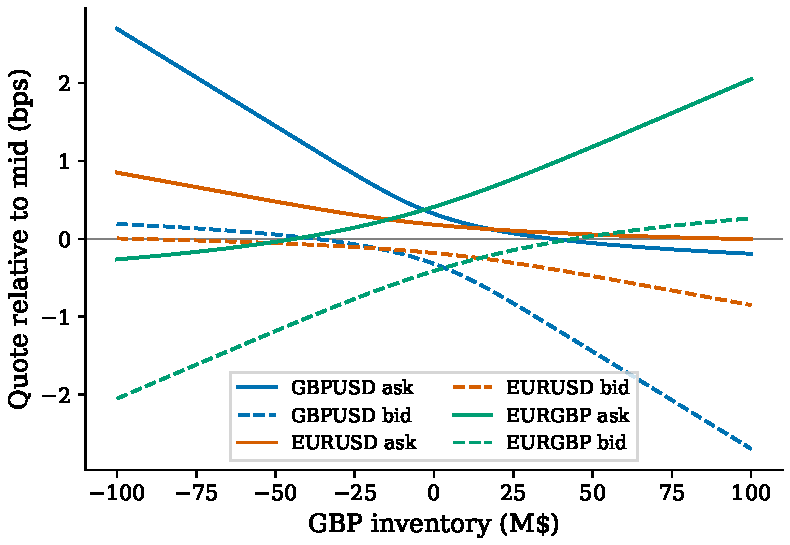
\includegraphics[width=0.85\textwidth]{figures/fig_ode_quotes_vs_inventory.pdf}
  \caption{Optimal top-of-book markups (tier 1, $z = 1$~M\$) for GBPUSD, EURUSD, and EURGBP as functions of GBP inventory, with other inventories at zero. Each pair shows bid and ask markups; the vertical distance between the two curves is the full spread. Risk aversion $\gamma = 20$~(M\$)$^{-1}$.}
  \label{fig:ode-quotes}
\end{figure}


% ------------------------------------------------------------------
\subsection{Optimal hedging}
\label{sec:ode-results-hedging}

Figure~\ref{fig:ode-hedging} shows the optimal hedge rates for all ten currency pairs as functions of EUR inventory, with all other inventories at zero. The figure reveals the structure of the dealer's externalization strategy.

The EURUSD hedge rate dominates: it is the primary channel for externalizing EUR inventory risk, which is natural since EURUSD is the most liquid pair with the lowest execution costs. The hedge rate is zero in an interval around zero inventory, forming the \emph{pure internalization zone} where the dealer prefers to manage risk entirely through price skewing rather than incurring the proportional spread cost~$\psi$ on the D2D market. Outside this zone, the hedge rate grows approximately linearly with inventory.

Other pairs also contribute to hedging, but at significantly lower rates. The correlated pairs (GBPUSD, CHFUSD, JPYUSD) are used to shed risk when the EUR inventory becomes large. This makes economic sense: when the EUR position is large, further price skewing on EURUSD alone has diminishing returns because the fill probability is already low, and the dealer can offload part of the correlated risk through other currency pairs. The cross pairs (EURGBP, EURCHF, EURJPY) also participate, providing additional hedging channels through which the dealer can trade EUR exposure against the non-USD currencies.

The inset in Figure~\ref{fig:ode-hedging} shows the correlation matrix of the five exchange rates, which drives the cross-currency hedging behavior. Pairs with higher correlation to EURUSD are used more actively for hedging EUR exposure.

\begin{figure}[t]
  \centering
  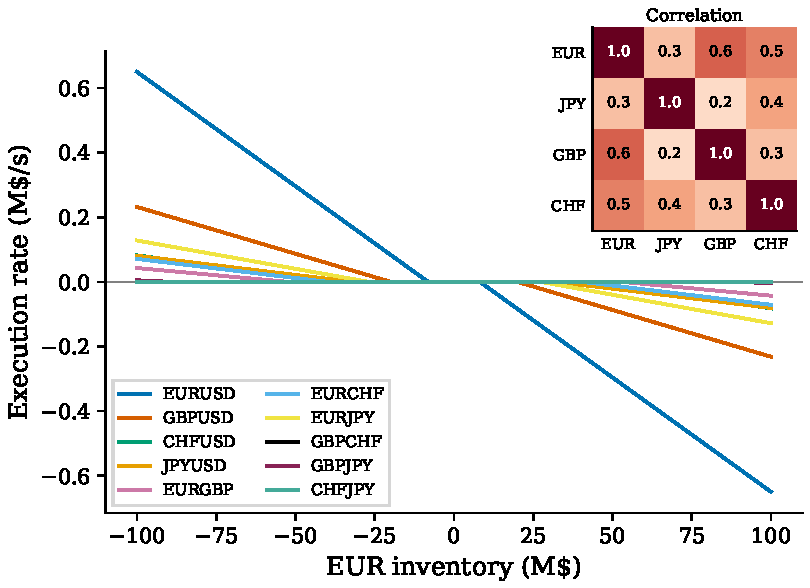
\includegraphics[width=0.85\textwidth]{figures/fig_ode_hedge_rates_vs_inventory.pdf}
  \caption{Optimal hedge rates for all ten currency pairs as functions of EUR inventory, with other inventories at zero. The pure internalization zone is visible around zero inventory for each pair. Inset: correlation matrix of the exchange rates. Risk aversion $\gamma = 20$~(M\$)$^{-1}$.}
  \label{fig:ode-hedging}
\end{figure}


% ------------------------------------------------------------------
\subsection{Inventory dynamics under the optimal strategy}
\label{sec:ode-results-mc}

To verify that the optimal strategy produces sensible inventory dynamics, we simulate the dealer's inventory process under the computed strategy using a tau-leaping Monte Carlo method. The simulation models client arrivals as Poisson events (with fill probabilities determined by the optimal markups) and hedging as a continuous drift, discretized over short time steps.

Figure~\ref{fig:ode-inventory} shows the resulting joint distribution of EUR and GBP inventories from a long simulation of the three-currency model (USD, EUR, GBP). The inventory distribution is approximately elliptical and concentrated around the origin, confirming that the strategy keeps the dealer's positions bounded. The contours of the risk function $\frac{\gamma}{2}\,y^\T\!\Sigma\,y$ are superimposed: the inventory distribution is clearly shaped by these risk contours, with the principal axis of the distribution aligned with the direction of minimum risk. This alignment arises because the dealer penalizes risk proportionally to $y^\T\!\Sigma\,y$ through the mean-variance term in the objective, and the optimal strategy acts to keep the inventory in the low-risk region.

The elongation of the distribution along the direction of positive EUR-GBP correlation reflects the fact that correlated positions partially offset each other in terms of portfolio risk. The dealer tolerates larger combined EUR-GBP positions when they are positively correlated (both long or both short) than when they are negatively correlated (long one, short the other), because the portfolio variance is lower in the former case.

\begin{figure}[t]
  \centering
  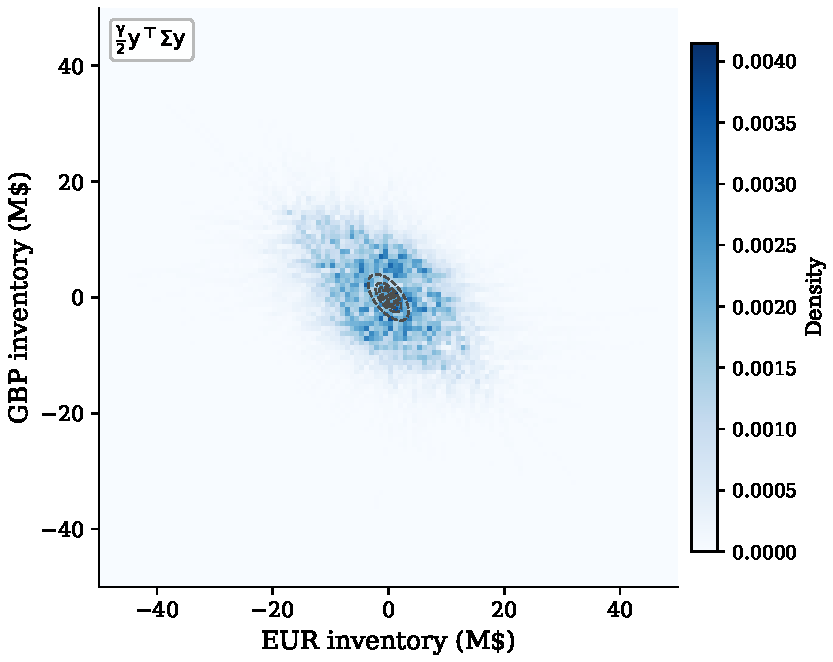
\includegraphics[width=0.7\textwidth]{figures/fig_ode_inventory_distribution.pdf}
  \caption{Joint distribution of EUR and GBP inventories under the optimal strategy in the three-currency model (USD, EUR, GBP), from a Monte Carlo simulation of $5 \times 10^5$ seconds. The 2D histogram of simulated inventories is overlaid with contours of constant portfolio risk $\frac{\gamma}{2}\,y^\T\!\Sigma\,y$. Risk aversion $\gamma = 20$~(M\$)$^{-1}$.}
  \label{fig:ode-inventory}
\end{figure}


% ------------------------------------------------------------------
\subsection{Discussion}
\label{sec:ode-results-discussion}

The numerical results illustrate three qualitative features of the multi-currency model that do not arise when each pair is treated in isolation.

First, \emph{cross-currency skewing}: the optimal markup on a given pair depends on the full inventory vector, not just the inventory in the pair's two currencies. This is visible in the EURUSD response to GBP inventory in Figure~\ref{fig:ode-quotes}. The strength of this cross-currency coupling is governed by the off-diagonal entries of~$A$, which in turn depend on correlations, cross-pair quoting activity, and the hedging cost structure.

Second, \emph{multi-pair hedging}: the dealer externalizes risk through a portfolio of D2D trades rather than hedging each pair independently. Figure~\ref{fig:ode-hedging} shows that even a purely EUR position induces hedge trades in multiple other pairs. This diversified hedging is more cost-effective than concentrating all externalization in a single pair, because the execution costs are pair-specific and the correlations allow partial risk transfer through correlated instruments.

Third, \emph{portfolio-level risk control}: the inventory distribution in Figure~\ref{fig:ode-inventory} is shaped by the risk contours of the full covariance matrix $\Sigma$, not by individual pair variances. The dealer manages risk at the portfolio level, tolerating larger positions when they are partially offsetting and keeping tighter control when positions compound each other.

These features are consistent with the findings reported in~\cite{barzykin2023} and confirm that our implementation of the ODE approximation reproduces the qualitative behavior of the paper's results. What remains to be established is the sensitivity of these results to the model parameters, which we investigate in Chapter~\ref{ch:sensitivity}, and the accuracy of the quadratic approximation against the full PDE solution, which is the subject of Chapter~\ref{ch:pde}.

\chapter{Sensitivity Analysis and Uncertainty Quantification}
\label{ch:sensitivity}

The ODE approximation developed in Chapter~\ref{ch:ode} computes the optimal market making strategy for a given set of model parameters in milliseconds. In practice, however, these parameters are not known exactly. Exchange rate volatilities fluctuate from day to day. Client arrival rates depend on market conditions. The logistic demand parameters $(\alpha_n, \beta_n)$ are fitted from historical fill-or-reject data via logistic regression and carry estimation error. The quadratic execution cost~$\eta$, which governs market impact in the hedging channel, is difficult to calibrate. The cross-pair correlation~$\rho$ is estimated from return data and varies across market regimes. Even the risk aversion~$\gamma$, which is a design choice rather than a market observable, is typically tuned rather than derived from first principles. A natural question is therefore: how sensitive is the optimal strategy to changes in these parameters, and how does parameter uncertainty propagate to the quantities that a market maker cares about?

We address this question through two complementary analyses. First, we use variance-based global sensitivity analysis \cite{sobol2001, saltelli2008} to decompose the output variance of each quantity of interest into contributions from individual parameters and their interactions. The resulting Sobol indices identify which parameters drive the uncertainty in each output and, equally important, which parameters can be safely fixed at nominal values. Second, we propagate the full parameter uncertainty forward through the model to obtain the probability distributions of the key strategy outputs, characterizing their spread and shape under realistic parameter ranges.

We work with three currencies (USD, EUR, GBP), the smallest setting that includes cross-pair correlations, cross-inventory effects on quoting, and cross-hedging. These are the multi-currency features that are central to the model of~\cite{barzykin2023} and that were demonstrated in Chapter~\ref{ch:ode}: the EURUSD markup shifts with GBP inventory (Figure~\ref{fig:ode-quotes}), the dealer hedges EUR exposure through multiple pairs (Figure~\ref{fig:ode-hedging}), and the inventory distribution is shaped by the full covariance structure (Figure~\ref{fig:ode-inventory}). Three currencies is the smallest setting that exhibits these mechanisms while remaining computationally tractable for a 220{,}000-evaluation Sobol study; adding more currencies would increase the parameter count but not introduce qualitatively new coupling mechanisms. With three currencies and three tradeable pairs, the model has 20 uncertain parameters and we define six quantities of interest that probe both the quoting policy and the hedging and economic outcomes.

The chapter is organized as follows. Section~\ref{sec:sa-setup} defines the parameters under study and the quantities of interest. Section~\ref{sec:sa-methodology} describes the Sobol index framework and the forward uncertainty quantification procedure. Sections~\ref{sec:sa-results-a} and~\ref{sec:sa-results-b} present the results for the quoting policy and the hedging and economic quantities, respectively. Section~\ref{sec:sa-discussion} discusses the overall sensitivity structure, identifies parameters that can be fixed, and assesses the robustness of the optimal strategy.


% ==================================================================
\section{Setup}
\label{sec:sa-setup}

% ------------------------------------------------------------------
\subsection{Parameters under study}
\label{sec:sa-params}

We study 20 parameters of the three-currency model: 5 global parameters that affect all pairs, and 5 pair-specific parameters for each of the three pairs (EURUSD, GBPUSD, EURGBP). Table~\ref{tab:sa-params} lists the parameters with their nominal values from Table~1 of~\cite{barzykin2023} and the ranges over which they are varied. All parameters are sampled from independent uniform distributions on their respective ranges.

\begin{table}[ht]
\centering
\caption{Parameters varied in the sensitivity analysis. Nominal values from Table~1 of~\cite{barzykin2023}. Ranges reflect realistic uncertainty around the nominal, chosen as $\pm 30$--$50\%$ for most parameters.}
\label{tab:sa-params}
\begin{tabular}{@{}clccc@{}}
\toprule
\# & Parameter & Symbol & Nominal & Range \\
\midrule
\multicolumn{5}{@{}l}{\textit{Global}} \\
1 & EUR volatility & $\sigma_{\text{EUR}}$ & 80\,bps & $[56,\; 104]$\,bps \\
2 & GBP volatility & $\sigma_{\text{GBP}}$ & 70\,bps & $[49,\; 91]$\,bps \\
3 & EUR/GBP correlation & $\rho$ & 0.6 & $[0.3,\; 0.9]$ \\
4 & Risk aversion & $\gamma$ & 20 & $[10,\; 40]$ \\
5 & Arrival rate scale & $\lambda_{\text{scale}}$ & 1.0 & $[0.5,\; 1.5]$ \\
\midrule
\multicolumn{5}{@{}l}{\textit{EUR/USD}} \\
6 & Logistic shift, tier 1 & $\alpha_1^{\text{EU}}$ & $-1.9$ & $[-2.5,\; -1.3]$ \\
7 & Logistic shift, tier 2 & $\alpha_2^{\text{EU}}$ & $-0.3$ & $[-0.9,\; 0.3]$ \\
8 & Logistic slope, tier 1 & $\beta_1^{\text{EU}}$ & $11.0$\,bps$^{-1}$ & $[7.7,\; 14.3]$ \\
9 & Logistic slope, tier 2 & $\beta_2^{\text{EU}}$ & $3.5$\,bps$^{-1}$ & $[2.45,\; 4.55]$ \\
10 & Execution cost & $\eta^{\text{EU}}$ & $10^{-5}$\,bps & $[0.5,\; 2.0] \times 10^{-5}$ \\
\midrule
\multicolumn{5}{@{}l}{\textit{GBP/USD}} \\
11 & Logistic shift, tier 1 & $\alpha_1^{\text{GU}}$ & $-1.4$ & $[-2.0,\; -0.8]$ \\
12 & Logistic shift, tier 2 & $\alpha_2^{\text{GU}}$ & $0.0$ & $[-0.6,\; 0.6]$ \\
13 & Logistic slope, tier 1 & $\beta_1^{\text{GU}}$ & $5.5$\,bps$^{-1}$ & $[3.85,\; 7.15]$ \\
14 & Logistic slope, tier 2 & $\beta_2^{\text{GU}}$ & $2.0$\,bps$^{-1}$ & $[1.4,\; 2.6]$ \\
15 & Execution cost & $\eta^{\text{GU}}$ & $1.5 \times 10^{-5}$\,bps & $[0.75,\; 3.0] \times 10^{-5}$ \\
\midrule
\multicolumn{5}{@{}l}{\textit{EUR/GBP}} \\
16 & Logistic shift, tier 1 & $\alpha_1^{\text{EG}}$ & $-0.5$ & $[-1.1,\; 0.1]$ \\
17 & Logistic shift, tier 2 & $\alpha_2^{\text{EG}}$ & $0.5$ & $[-0.1,\; 1.1]$ \\
18 & Logistic slope, tier 1 & $\beta_1^{\text{EG}}$ & $3.5$\,bps$^{-1}$ & $[2.45,\; 4.55]$ \\
19 & Logistic slope, tier 2 & $\beta_2^{\text{EG}}$ & $2.5$\,bps$^{-1}$ & $[1.75,\; 3.25]$ \\
20 & Execution cost & $\eta^{\text{EG}}$ & $3 \times 10^{-5}$\,bps & $[1.5,\; 6.0] \times 10^{-5}$ \\
\bottomrule
\end{tabular}
\end{table}

The volatilities~$\sigma$ and arrival rate scale~$\lambda_{\text{scale}}$ are estimated from market data and fluctuate with market conditions. The logistic demand parameters $(\alpha_n, \beta_n)$ are fitted from historical fill-or-reject data for each client tier on each pair and carry estimation error. The risk aversion~$\gamma$ is a design choice but is tuned in practice, so treating it as uncertain captures the sensitivity of the strategy to this subjective input. The execution cost~$\eta$ governs market impact in the hedging channel and is hard to estimate precisely. The correlation~$\rho$ between EUR and GBP exchange rates is estimated from return data and varies across market regimes; it controls the strength of cross-pair coupling through the covariance matrix~$\Sigma$.

The arrival rates for the five trade sizes are not varied independently but are scaled by a single shared multiplier~$\lambda_{\text{scale}}$ applied uniformly across all three pairs. This reflects the realistic scenario that overall market activity rises or falls broadly. The demand curve and execution cost parameters, by contrast, are varied independently per pair, since each pair has a distinct client base and liquidity profile.

Several parameters are held fixed at their nominal values: the linear execution cost~$\psi$ (set by the execution desk and relatively well known), the terminal penalty~$\kappa$ (set to zero in the paper's example), the time horizon $T = 0.05$\,days, the drift~$\mu$ (zero in the paper's example), and the exogenous trade rates~$k_i$ (negligibly small). These parameters are expected to have at most a local effect on the strategy, and excluding them keeps the analysis focused on the 20 inputs with genuine uncertainty or design freedom.


% ------------------------------------------------------------------
\subsection{Quantities of interest}
\label{sec:sa-qois}

For each parameter sample, we solve the Riccati ODE system of Chapter~\ref{ch:ode} and extract six scalar quantities of interest (QoIs). All six are deterministic given the ODE solution and introduce no sampling noise. We organize them into two groups: Set~A probes the quoting policy, the quantities that determine what the client sees; Set~B probes hedging and economic outcomes, the quantities that the trading desk manages.

The QoIs are evaluated at three inventory states, each a single-currency perturbation from flat:
\[
  y_{\text{flat}} = (0, 0, 0), \qquad y_{\text{long EUR}} = (0, 10, 0)\;\text{M\$}, \qquad y_{\text{long GBP}} = (0, 0, 10)\;\text{M\$}.
\]
Using single-currency perturbations isolates the own-inventory and cross-inventory mechanisms cleanly.

\paragraph{Set A: quoting policy.}

\begin{enumerate}
  \item \textbf{Tier spread differential} (bps). The difference in optimal markups between tier~1 (aggressive) and tier~2 (passive) on EURUSD at flat inventory, for trade size $z = 1$\,M\$:
  \[
    \text{QoI}_1 = \delta^*(y_{\text{flat}},\; \text{tier 1}) - \delta^*(y_{\text{flat}},\; \text{tier 2}).
  \]
  This measures the basis of client-tiered pricing: how much wider the model quotes for passive clients. Since tier~2 has a less price-sensitive demand curve, the tier~2 markup exceeds the tier~1 markup, making this quantity negative.

  \item \textbf{Own-inventory skew} (bps). The change in the tier~1 EURUSD markup when the dealer holds 10\,M\$ in EUR:
  \[
    \text{QoI}_2 = \delta^*(y_{\text{long EUR}},\; \text{tier 1}) - \delta^*(y_{\text{flat}},\; \text{tier 1}).
  \]
  This measures the strategy's responsiveness to own-pair inventory risk, the skewing behavior visible in the EURUSD panel of Figure~\ref{fig:ode-quotes}.

  \item \textbf{Cross-inventory skew} (bps). The change in the tier~1 EURUSD markup when the dealer holds 10\,M\$ in GBP instead:
  \[
    \text{QoI}_3 = \delta^*(y_{\text{long GBP}},\; \text{tier 1}) - \delta^*(y_{\text{flat}},\; \text{tier 1}).
  \]
  It measures the cross-currency influence demonstrated in Figure~\ref{fig:ode-quotes}, where EURUSD quotes shift with GBP inventory through the off-diagonal entries of the Riccati matrix~$A$.
\end{enumerate}

\paragraph{Set B: hedging and economics.}

\begin{enumerate}
  \setcounter{enumi}{3}
  \item \textbf{Own-pair hedge rate} (M\$/s). The optimal EURUSD hedge rate when holding 10\,M\$ in EUR:
  \[
    \text{QoI}_4 = \xi^*_{\text{EURUSD}}(y_{\text{long EUR}}).
  \]
  This measures how aggressively the model externalizes EUR inventory risk through the dealer-to-dealer market, the hedging channel analyzed in Figure~\ref{fig:ode-hedging}.

  \item \textbf{Cross-hedge momentum} (decimal). The value function gradient projected onto the EURGBP hedging direction at the long-EUR inventory:
  \[
    \text{QoI}_5 = p_{\text{EURGBP}} = -(2A(0)\,y_{\text{long EUR}} + B(0))^\T d_{\text{EUR,GBP}}.
  \]
  This is the ``desire to cross-hedge'': the momentum that would drive EURGBP hedging if execution costs were zero. We use the raw momentum rather than the clipped hedge rate $\xi^*_{\text{EURGBP}}$ because the EURGBP dead zone ($\psi_{\text{EG}} = 0.25$\,bps) exceeds the typical momentum magnitude for nearly all parameter samples, leaving the actual hedge rate at zero with insufficient variance for meaningful Sobol decomposition. The momentum is continuous, well-behaved, and reveals the sensitivity structure of the cross-hedging incentive.

  \item \textbf{Net revenue} (\$/day). Total expected revenue from quoting across all three pairs minus total hedging cost, at the long-EUR inventory:
  \[
    \text{QoI}_6 = R(y_{\text{long EUR}}) - L_{\text{total}}(y_{\text{long EUR}}),
  \]
  where $R = \sum_{\text{pairs, directions, tiers, sizes}} \lambda_k\,f(\delta^*)\,\delta^*\,z_k$ is the instantaneous revenue rate and $L_{\text{total}} = \sum_{\text{pairs}} (\psi\,|\xi^*| + \eta\,(\xi^*)^2)$ is the total hedging cost. This is the bottom line under inventory pressure: ``given that the desk is carrying EUR inventory, is it making money after hedging costs?''
\end{enumerate}

QoIs~1, 2, and~4 measure own-pair quantities that depend on a single currency pair's parameters and the global market environment. QoIs~3 and~5 measure cross-pair quantities that depend on the correlation and volatility parameters coupling different pairs. QoI~6 integrates across all pairs. This mix lets us test whether cross-currency coupling introduces new sensitivity dimensions beyond the own-pair parameters.


% ==================================================================
\section{Methodology}
\label{sec:sa-methodology}

% ------------------------------------------------------------------
\subsection{Sobol indices}
\label{sec:sa-sobol-method}

We use variance-based global sensitivity analysis to quantify how much of the output variance in each QoI is attributable to each input parameter. The framework, introduced by Sobol~\cite{sobol2001} and developed by Saltelli et al.~\cite{saltelli2008}, decomposes the variance of a model output $Y = g(X_1, \ldots, X_k)$ into contributions from individual inputs and their interactions.

The \emph{first-order Sobol index} $S_i$ measures the fraction of the total output variance explained by parameter~$X_i$ alone, averaging over all other parameters:
\begin{equation}
  \label{eq:sobol-first}
  S_i = \frac{\operatorname{Var}_{X_i}\!\bigl(\E_{X_{\sim i}}[Y \mid X_i]\bigr)}{\operatorname{Var}(Y)},
\end{equation}
where $X_{\sim i}$ denotes all parameters except~$X_i$. The \emph{total-effect index} $S_{T_i}$ captures all contributions involving~$X_i$, whether individually or through interactions:
\begin{equation}
  \label{eq:sobol-total}
  S_{T_i} = 1 - \frac{\operatorname{Var}_{X_{\sim i}}\!\bigl(\E_{X_i}[Y \mid X_{\sim i}]\bigr)}{\operatorname{Var}(Y)}.
\end{equation}
If $S_{T_i} \approx 0$, the parameter has no effect on the output and can be safely fixed at any value within its range. If $S_{T_i} \gg S_i$, the parameter participates in important interactions with other parameters. A model is additive when each parameter's effect on the output does not depend on the values of the other parameters; equivalently, $S_i = S_{T_i}$ for every~$i$. When the model is perfectly additive, the first-order indices sum to one, while interactions cause $\sum_i S_i < 1$ and $\sum_i S_{T_i} > 1$, since the shared variance is counted once per participating parameter in the total-effect indices.

We estimate the indices using the Monte Carlo procedure of Saltelli et al.~\cite{saltelli2010}, with the total-effect estimator of Jansen~\cite{jansen1999}. The algorithm proceeds as follows.
\begin{enumerate}
  \item Draw two independent sample matrices $\mathbf{A}$ and $\mathbf{B}$ of shape $(N, k)$, where $N$ is the number of base samples and $k = 20$. Each row is drawn uniformly from the parameter ranges in Table~\ref{tab:sa-params}.
  \item For each parameter $i = 1, \ldots, k$, construct $\mathbf{C}_i$ by taking $\mathbf{A}$ and replacing its $i$-th column with the corresponding column from~$\mathbf{B}$.
  \item Evaluate the model at all $N(k+2)$ sample points: $N$~rows of~$\mathbf{A}$, $N$~rows of~$\mathbf{B}$, and $N$~rows of each~$\mathbf{C}_i$.
  \item Compute the indices from the sample covariances:
  \begin{align}
    \label{eq:sobol-estimators}
    S_i &= \frac{\frac{1}{N}\sum_{j=1}^{N} g(\mathbf{B}_j)\bigl(g(\mathbf{C}_i^{(j)}) - g(\mathbf{A}_j)\bigr)}{\widehat{\operatorname{Var}}(Y)}, \\[4pt]
    S_{T_i} &= \frac{\frac{1}{2N}\sum_{j=1}^{N}\bigl(g(\mathbf{A}_j) - g(\mathbf{C}_i^{(j)})\bigr)^2}{\widehat{\operatorname{Var}}(Y)},
  \end{align}
  where $\widehat{\operatorname{Var}}(Y)$ is the sample variance over the combined $\mathbf{A}$ and $\mathbf{B}$ evaluations.
\end{enumerate}

We use $N = 10{,}000$ base samples, giving $10{,}000 \times 22 = 220{,}000$ model evaluations. Each evaluation solves the $3 \times 3$ Riccati ODE system with 500 Euler steps, which takes approximately 12\,ms on a standard computer, for a total computation time of about 45 minutes. This analysis is feasible only because of the ODE approximation; the PDE solver developed in Chapter~\ref{ch:pde} requires on the order of minutes per evaluation, making a comparable 220{,}000-evaluation study computationally prohibitive. The same Sobol-based methodology has been applied to ODE-based models in other contexts; see~\cite{jakobsson2023, piazzola2021} for applications to epidemiological compartment models.


% ------------------------------------------------------------------
\subsection{Forward uncertainty quantification}
\label{sec:sa-forward-method}

After identifying the important parameters through the Sobol analysis, we characterize the full output distributions by propagating the parameter uncertainty forward through the model. Rather than generating new samples, we reuse the $2N = 20{,}000$ evaluations from the Sobol computation (the $\mathbf{A}$ and $\mathbf{B}$ samples), which are already drawn from the uniform prior distributions specified in Table~\ref{tab:sa-params}.

For each QoI, we estimate the probability density function using Gaussian kernel density estimation with Silverman's rule for bandwidth selection, and report the mean, standard deviation, coefficient of variation (CV), and 90\% credible interval (5th to 95th percentile). The coefficient of variation, defined as the ratio of the standard deviation to the absolute value of the mean, provides a scale-free measure of output robustness: a small CV indicates that the output is stable under parameter uncertainty, while a large CV signals that the model's prescription is highly sensitive to the input values.


% ==================================================================
\section{Results: quoting policy (Set A)}
\label{sec:sa-results-a}

Before examining each QoI individually, Figure~\ref{fig:sa-heatmap} presents the total-effect Sobol indices for all 20 parameters and all 6 QoIs in a single heatmap. The block structure is immediately visible: the EUR/USD demand parameters (rows~6--9) light up only for QoI~1, the global market parameters (rows~1--5) dominate QoIs~2--5, and $\lambda_{\text{scale}}$ alone dominates QoI~6. The GBP/USD and EUR/GBP pair-specific parameters (rows~11--20) are near-zero across all QoIs. This pattern, which the following subsections examine in detail, reflects a clean separation between the microstructure parameters that control client pricing and the market-level parameters that control risk management.

\begin{figure}[t]
  \centering
  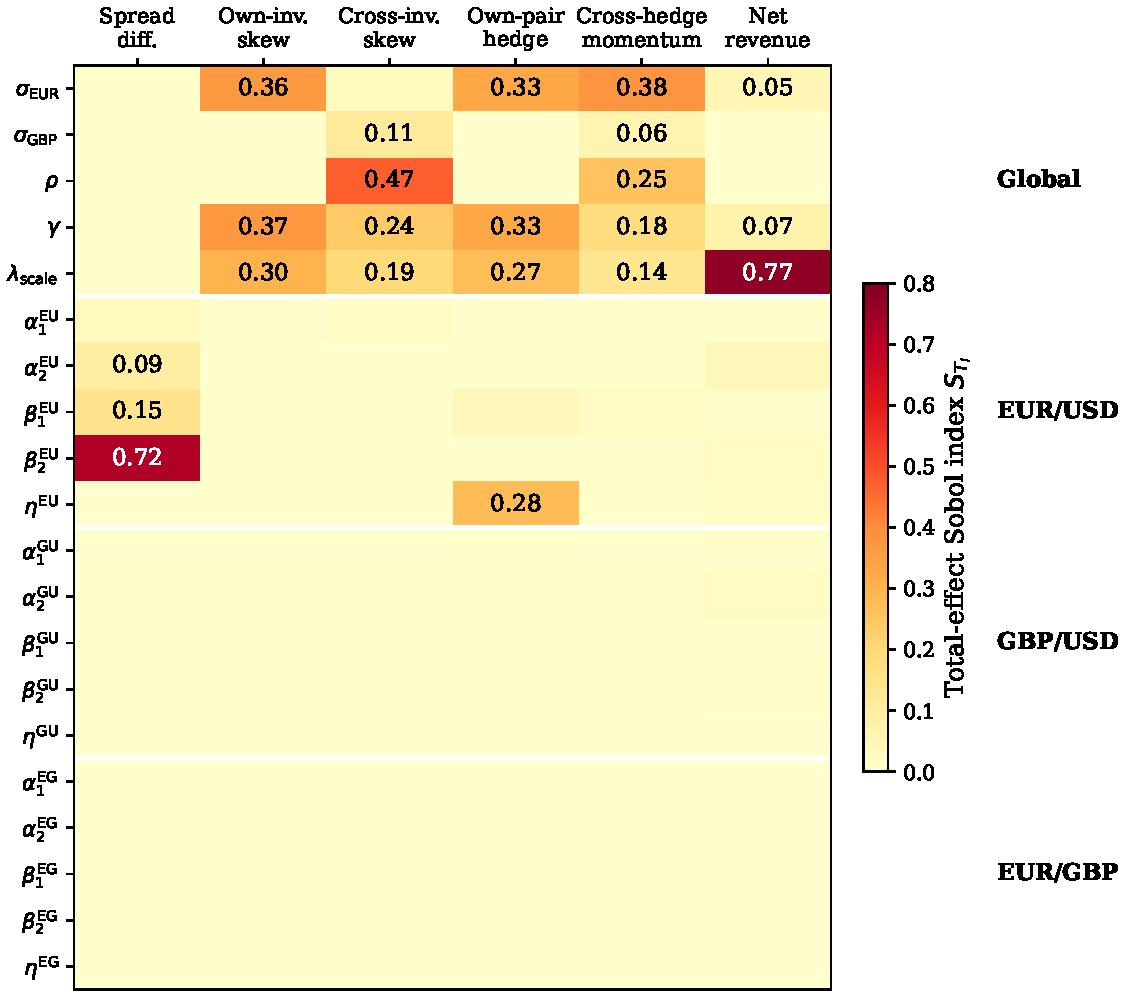
\includegraphics[width=0.75\textwidth]{figures/fig_sa_heatmap.pdf}
  \caption{Total-effect Sobol indices $S_{T_i}$ for 20 parameters (rows) and 6 quantities of interest (columns). Values above 0.05 are annotated. Parameters are grouped into global, EUR/USD, GBP/USD, and EUR/GBP. The block structure shows that different QoIs are sensitive to different parameter groups.}
  \label{fig:sa-heatmap}
\end{figure}


% ------------------------------------------------------------------
\subsection{Tier spread differential}
\label{sec:sa-qoi1}

The tier spread differential measures how much wider the model quotes for passive clients (tier~2) compared to aggressive clients (tier~1) on EURUSD at flat inventory. Figure~\ref{fig:sa-qoi1} shows the Sobol indices and output distribution.

\begin{figure}[ht]
  \centering
  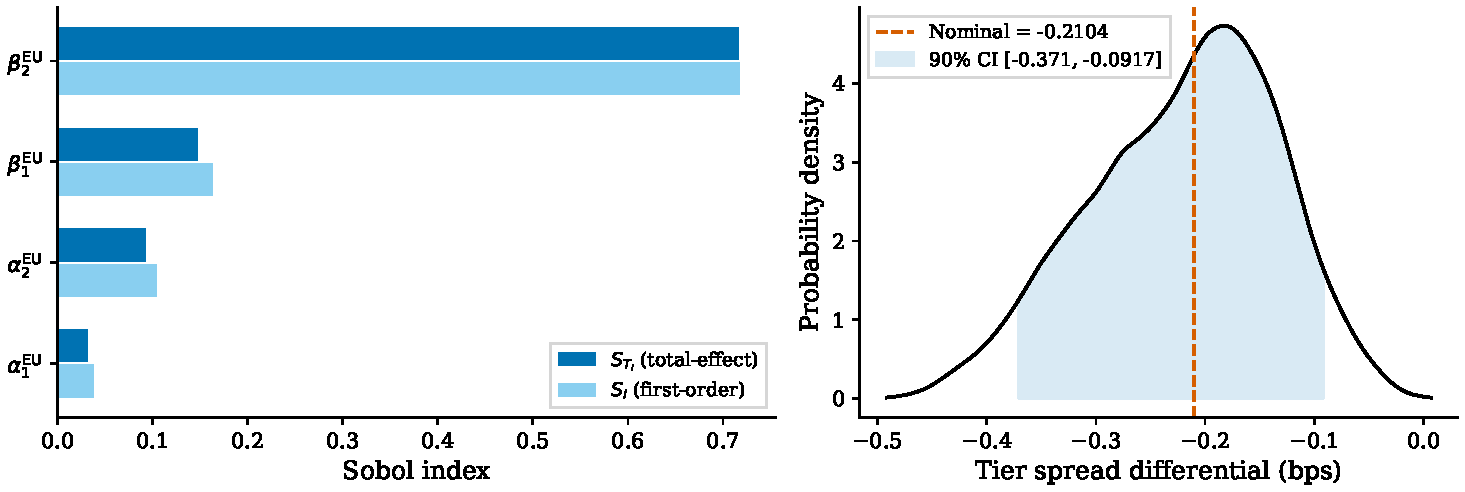
\includegraphics[width=\textwidth]{figures/fig_sa_qoi1.pdf}
  \caption{QoI~1: tier spread differential. Left: Sobol indices for parameters with $S_{T_i} > 0.02$. Right: output distribution from forward UQ ($n = 20{,}000$ samples), with nominal value (dashed red) and 90\% credible interval (shaded).}
  \label{fig:sa-qoi1}
\end{figure}

The tier spread differential is controlled entirely by the EUR/USD demand curve parameters. The passive-tier logistic slope $\beta_2^{\text{EU}}$ dominates ($S_i = 0.72$, $S_{T_i} = 0.72$), followed by $\beta_1^{\text{EU}}$ ($S_i = 0.17$, $S_{T_i} = 0.15$), $\alpha_2^{\text{EU}}$ ($S_i = 0.11$, $S_{T_i} = 0.09$), and $\alpha_1^{\text{EU}}$ ($S_i = 0.04$, $S_{T_i} = 0.03$). All other parameters, including all global parameters and all GBP/USD and EUR/GBP parameters, have $S_{T_i} < 0.001$. The first-order indices sum to 1.03 and the total-effect indices to 0.99; both estimates bracket 1 within Monte Carlo noise at $N = 10{,}000$, consistent with a perfectly additive model.

This result follows from the structure of the quoting formula. At zero inventory with $B(0) = 0$ (which holds under the direction-symmetric parameters of~\cite{barzykin2023}), the quoting momentum~\eqref{eq:p-formula} reduces to $p = z\,d^\T A(0)\,d$, which is small for the trade size $z = 1$\,M\$ considered here. The optimal markup is therefore dominated by the maximization of $f^n(\delta) \cdot \delta$ over the logistic demand curve, which depends only on the $(\alpha_n, \beta_n)$ of the two tiers being compared. The Riccati matrix $A(0)$ does depend on $\sigma$, $\gamma$, $\rho$, and $\lambda$ through the full dynamics~\eqref{eq:riccati-A}, but its contribution to the momentum~$p$ is negligible at this trade size.

A bank seeking to control its tiered client pricing therefore needs only to estimate the demand curves accurately. Volatility, risk aversion, and all cross-pair parameters are irrelevant for the flat-inventory spread differential. The forward UQ confirms moderate uncertainty (mean $= -0.22$\,bps, CV $= 39\%$, 90\% CI $= [-0.37, -0.09]$\,bps), reflecting the estimation error in the demand curve parameters.


% ------------------------------------------------------------------
\subsection{Own-inventory skew}
\label{sec:sa-qoi2}

The own-inventory skew measures how the EURUSD markup adjusts when the dealer holds 10\,M\$ in EUR. Figure~\ref{fig:sa-qoi2} shows the results.

\begin{figure}[ht]
  \centering
  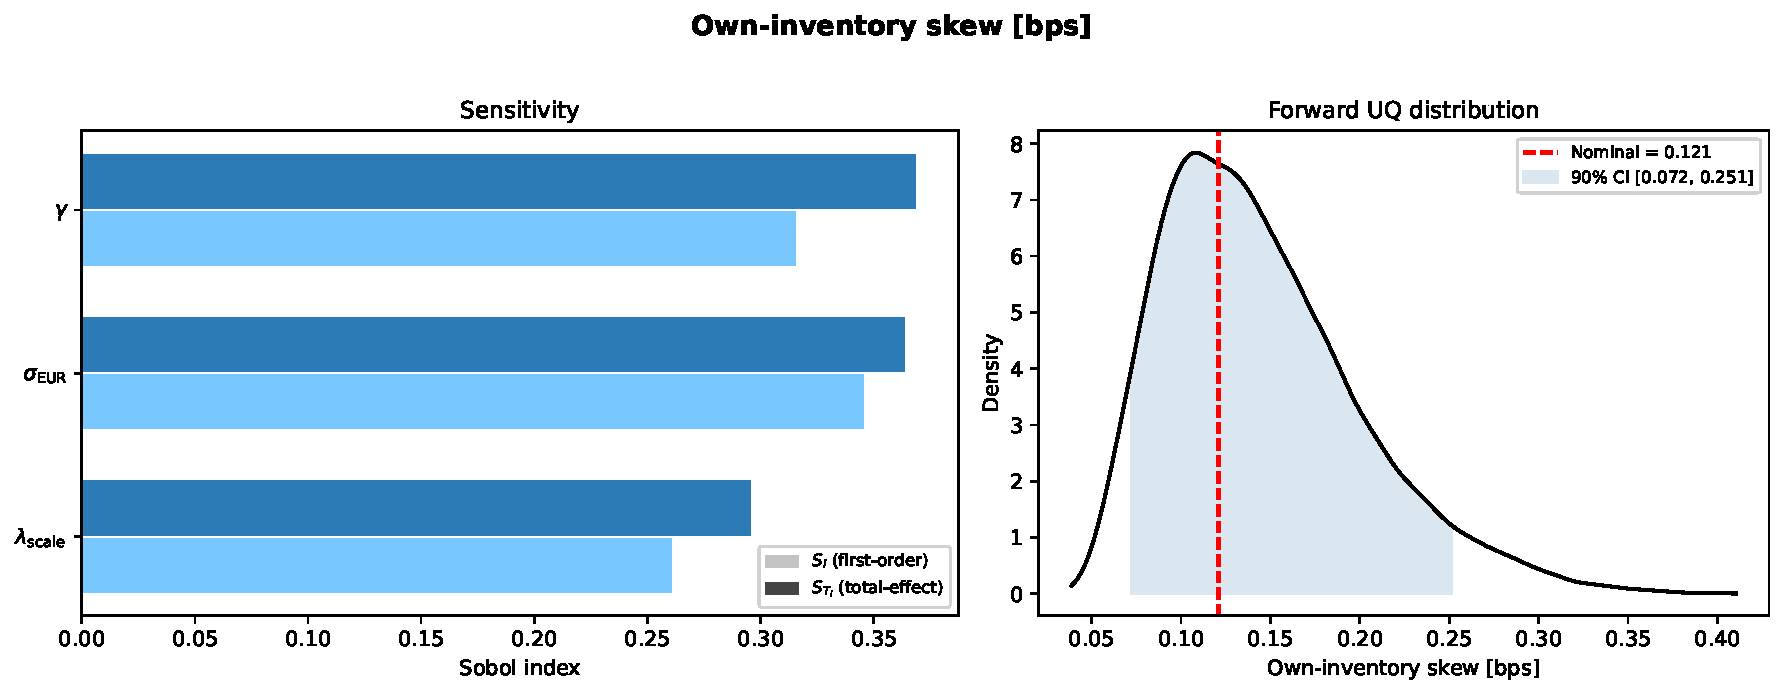
\includegraphics[width=\textwidth]{figures/fig_sa_qoi2.pdf}
  \caption{QoI~2: own-inventory skew. Left: Sobol indices. Right: output distribution.}
  \label{fig:sa-qoi2}
\end{figure}

The inventory skew is driven by three global parameters with roughly equal importance: $\sigma_{\text{EUR}}$ ($S_i = 0.35$, $S_{T_i} = 0.36$), $\gamma$ ($S_i = 0.32$, $S_{T_i} = 0.37$), and $\lambda_{\text{scale}}$ ($S_i = 0.26$, $S_{T_i} = 0.30$). All pair-specific parameters and the cross-pair parameters ($\sigma_{\text{GBP}}$, $\rho$) have $S_{T_i} < 0.01$. The model is nearly additive ($\sum S_i = 0.94$, $\sum S_{T_i} = 1.05$).

The skew arises from the value function gradient $2A(0)\,y$, and each of the three dominant parameters shapes the Riccati solution~$A$ through a different channel. Higher volatility increases inventory risk through the driving term $-\tfrac{\gamma}{2}\Sigma$ in~\eqref{eq:riccati-A}, enlarging~$A$ and hence the skew. Higher risk aversion amplifies this driving term directly. Higher arrival rates change the structure of the quoting Hamiltonian coefficients that enter the nonlinear term $2AMA$ in~\eqref{eq:riccati-A}, altering how the model balances quoting revenue against inventory risk. The demand curve parameters $(\alpha_n, \beta_n)$ affect the level of the spread but not its inventory dependence, because they enter through the Hamiltonian Taylor coefficients which scale~$A$ approximately uniformly.

The cross-pair parameters $\rho$ and $\sigma_{\text{GBP}}$ do not appear, even though they affect the diagonal entry $A_{\text{EUR,EUR}}$ through the Riccati coupling. The coupling's effect on the own-pair diagonal entries of~$A$ is too small to register at this sample size. The inventory adjustment of a single pair depends on the market environment (volatility, overall flow, risk preference) and is insensitive to the client demand model.

Forward UQ: mean $= 0.15$\,bps, CV $= 38\%$, 90\% CI $= [0.07, 0.25]$\,bps. The nominal value of 0.12\,bps falls below the mean because the uniform range for~$\gamma$ ($[10, 40]$, midpoint 25) lies above the nominal value of 20, pulling the average skew upward.


% ------------------------------------------------------------------
\subsection{Cross-inventory skew}
\label{sec:sa-qoi3}

The cross-inventory skew measures how GBP inventory shifts the EURUSD markup, probing the cross-currency coupling through the off-diagonal entries of~$A$. Figure~\ref{fig:sa-qoi3} shows the results.

\begin{figure}[ht]
  \centering
  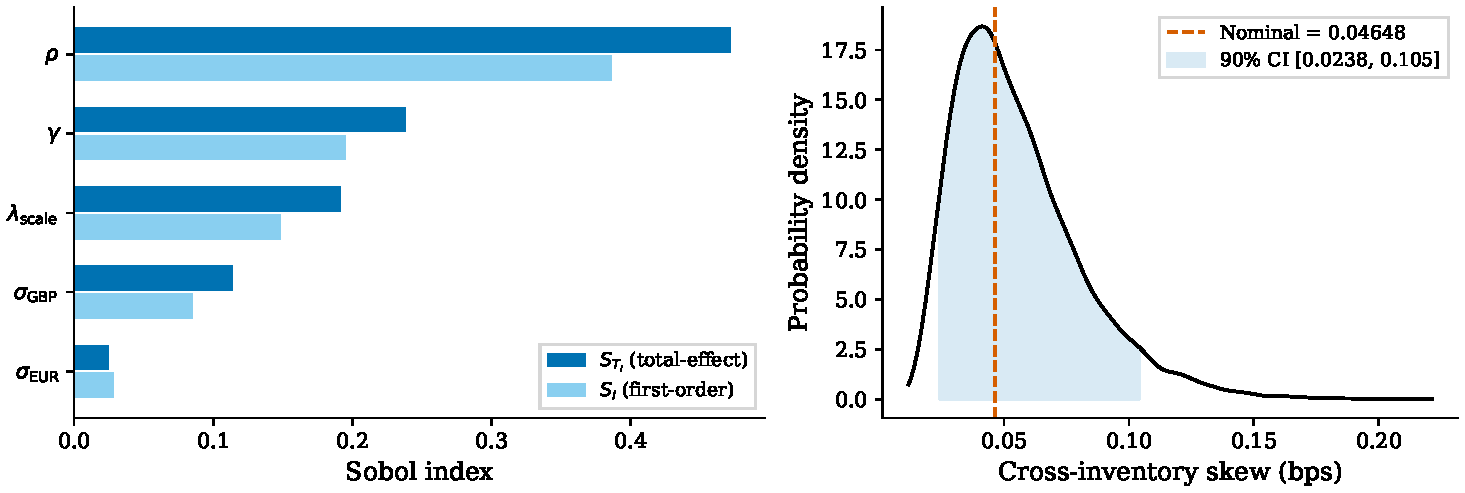
\includegraphics[width=\textwidth]{figures/fig_sa_qoi3.pdf}
  \caption{QoI~3: cross-inventory skew. Left: Sobol indices. Right: output distribution. The 90\% CI is entirely positive, confirming that the cross-pair coupling is a structural feature, not noise.}
  \label{fig:sa-qoi3}
\end{figure}

The cross-inventory skew is primarily driven by the correlation $\rho$ ($S_i = 0.39$, $S_{T_i} = 0.47$), confirming that correlation is the gateway to all cross-pair effects. The risk aversion~$\gamma$ ($S_i = 0.20$, $S_{T_i} = 0.24$) and arrival rate scale $\lambda_{\text{scale}}$ ($S_i = 0.15$, $S_{T_i} = 0.19$) are secondary drivers. The GBP volatility $\sigma_{\text{GBP}}$ appears at a lower level ($S_i = 0.09$, $S_{T_i} = 0.12$), and EUR volatility $\sigma_{\text{EUR}}$ registers a minor contribution. The gap between $S_i$ and $S_{T_i}$ for $\rho$ (0.39 vs.\ 0.47) indicates moderate interaction with the other global parameters. The total-effect indices sum to 1.08, so the model is nearly additive with a modest interaction contribution concentrated on~$\rho$.

The cross-inventory skew depends on the off-diagonal entries of~$A$ that couple GBP to the EUR/USD quoting momentum. These entries arise from the correlation entering the Riccati driving term $-\tfrac{\gamma}{2}\Sigma$: the off-diagonal covariance is $\Sigma_{\text{EUR,GBP}} = \rho\,\sigma_{\text{EUR}}\,\sigma_{\text{GBP}}$, so when $\rho = 0$ the off-diagonal of~$\Sigma$ vanishes, $A_{\text{EUR,GBP}} = 0$, and the cross-skew is zero. The GBP volatility $\sigma_{\text{GBP}}$ enters for the same reason: it scales the off-diagonal covariance that generates the cross-pair coupling.

One might expect that demand parameters of one pair could affect the strategy for another pair, since the Riccati matrices $M$, $\tilde{M}$, and $P$ aggregate Hamiltonian coefficients from all three pairs. The Sobol analysis shows that this coupling is negligible: no cross-pair demand parameter has $S_{T_i} > 0.015$ for the cross-inventory skew. Cross-pair effects propagate through the covariance matrix, not through client flow characteristics.

The forward UQ shows a mean cross-skew of 0.055\,bps with CV $= 46\%$ and a 90\% CI of $[0.024, 0.105]$\,bps. The CI is entirely positive: the cross-pair coupling is consistently nonzero across the parameter space. The magnitude is about 38\% of the own-inventory skew (mean 0.15\,bps), confirming that cross-pair coupling is a genuine structural feature of the multi-currency model, large enough to be practically relevant for a bank managing multiple currency desks.


% ==================================================================
\section{Results: hedging and economics (Set B)}
\label{sec:sa-results-b}


% ------------------------------------------------------------------
\subsection{Own-pair hedge rate}
\label{sec:sa-qoi4}

The own-pair hedge rate measures how aggressively the model hedges EUR exposure through the EURUSD interbank market. Figure~\ref{fig:sa-qoi4} shows the results.

\begin{figure}[ht]
  \centering
  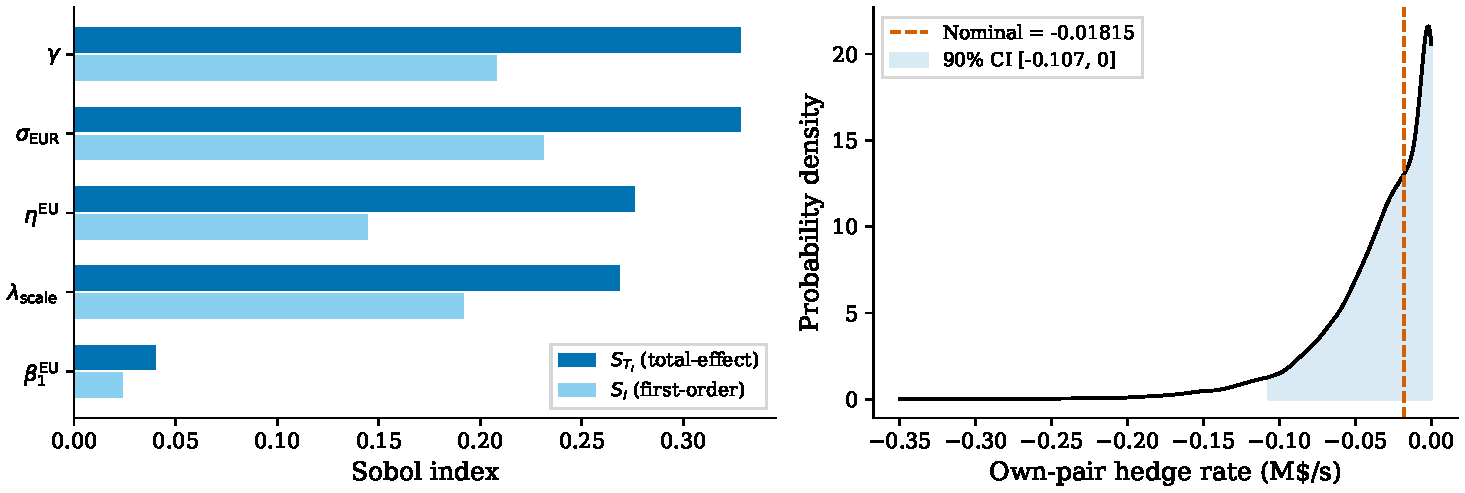
\includegraphics[width=\textwidth]{figures/fig_sa_qoi4.pdf}
  \caption{QoI~4: own-pair hedge rate. Left: Sobol indices, showing the largest gap between $S_i$ and $S_{T_i}$ for~$\eta^{\text{EU}}$ (strong interactions). Right: output distribution, with CV $= 111\%$.}
  \label{fig:sa-qoi4}
\end{figure}

Four parameters contribute: $\sigma_{\text{EUR}}$ ($S_i = 0.23$, $S_{T_i} = 0.33$), $\gamma$ ($S_i = 0.21$, $S_{T_i} = 0.33$), $\lambda_{\text{scale}}$ ($S_i = 0.19$, $S_{T_i} = 0.27$), and $\eta^{\text{EU}}$ ($S_i = 0.15$, $S_{T_i} = 0.28$). No cross-pair parameter has $S_{T_i} > 0.01$. The total-effect indices sum to 1.26, the highest of any QoI, indicating significant interaction effects.

The interactions arise from the hedge rate formula. Outside the dead zone, $\xi^* = (p - \psi)/(2\eta)$, where the hedging momentum~$p$ depends on the value function gradient and hence on $\sigma$, $\gamma$, and~$\lambda$ through the Riccati solution. The execution cost~$\eta$ enters multiplicatively with~$p$: changing~$\eta$ amplifies or dampens the effect of every parameter that influences the gradient. This multiplicative coupling explains why $\eta^{\text{EU}}$ has the largest gap between $S_i$ and $S_{T_i}$ ($0.15$ vs.\ $0.28$, a ratio of nearly 2).

The cross-pair parameters do not affect own-pair hedging. Although the model has EURGBP available as an alternative hedge instrument, the EURGBP dead zone blocks cross-hedging for nearly all parameter combinations (see QoI~5 below), so the EURUSD hedge rate is determined as if it were the only hedging channel.

The forward UQ confirms that the hedge rate is the least robust component of the strategy: mean $= -0.0335$\,M\$/s, standard deviation $= 0.0372$, CV $= 111\%$, 90\% CI $= [-0.107,\; 0]$\,M\$/s. The CI spans more than an order of magnitude. The distribution is heavily left-skewed because small values of~$\eta$ produce extremely large hedge rates through the $1/(2\eta)$ factor. The upper end of the CI reaches zero, meaning that for some parameter combinations the hedging momentum falls within the dead zone and the model prescribes no hedging at all.


% ------------------------------------------------------------------
\subsection{Cross-hedge momentum}
\label{sec:sa-qoi5}

Chapter~\ref{ch:ode} showed that the model hedges EUR exposure through multiple pairs, including the cross pair EURGBP (Figure~\ref{fig:ode-hedging}). To measure the sensitivity of this cross-hedging channel, we examine the value function's incentive to cross-hedge: the raw hedging momentum~$p_{\text{EURGBP}}$ before the dead zone clips it. Figure~\ref{fig:sa-qoi5} shows the results.

\begin{figure}[ht]
  \centering
  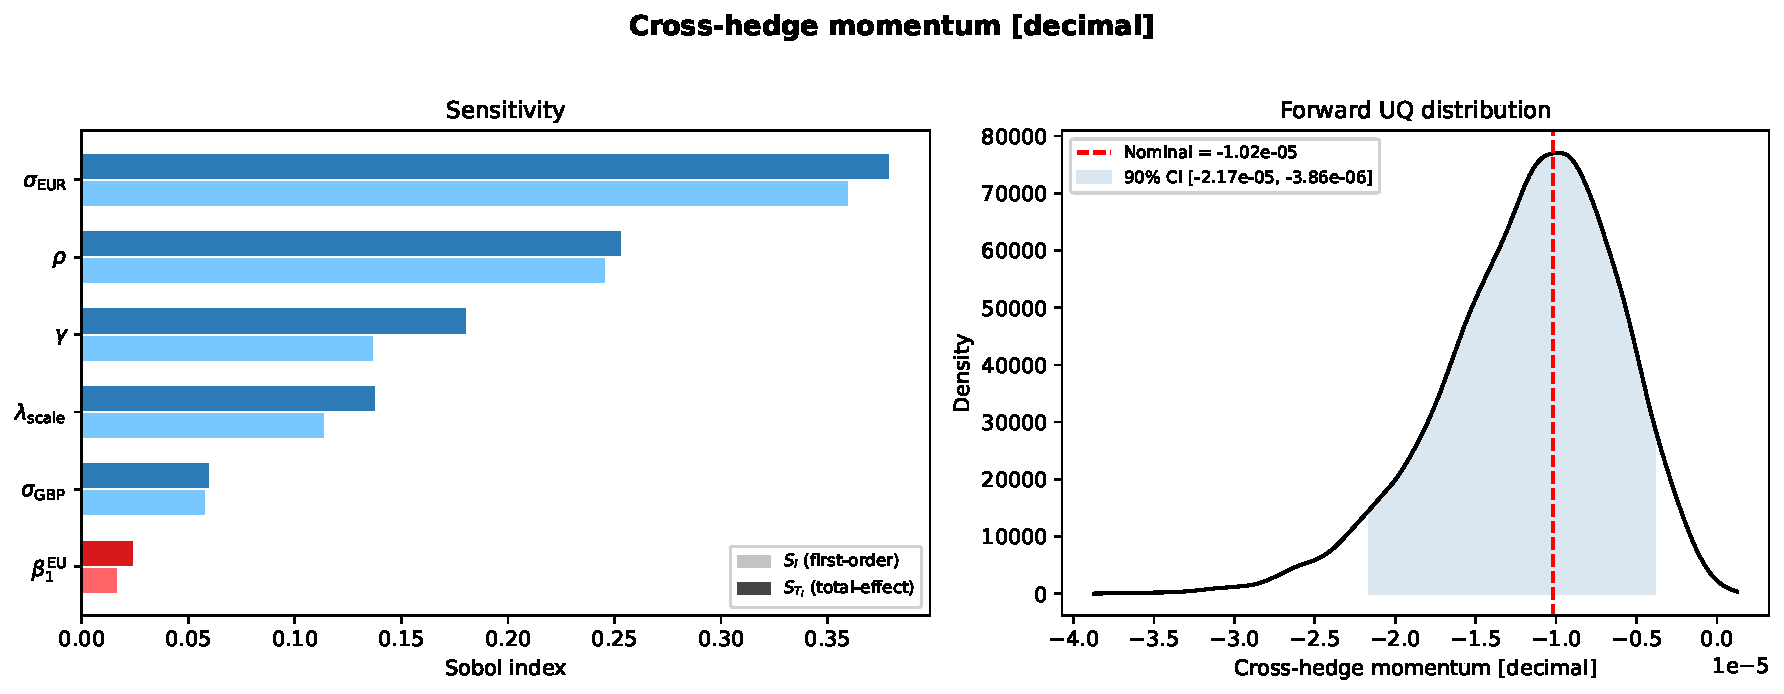
\includegraphics[width=\textwidth]{figures/fig_sa_qoi5.pdf}
  \caption{QoI~5: cross-hedge momentum. Left: Sobol indices. Right: output distribution. The momentum is consistently negative (the model wants to sell EUR / buy GBP to hedge), but its magnitude is smaller than the EURGBP dead zone.}
  \label{fig:sa-qoi5}
\end{figure}

The cross-hedge momentum is driven entirely by global parameters: $\sigma_{\text{EUR}}$ ($S_i = 0.36$, $S_{T_i} = 0.38$), $\rho$ ($S_i = 0.25$, $S_{T_i} = 0.25$), $\gamma$ ($S_i = 0.14$, $S_{T_i} = 0.18$), $\lambda_{\text{scale}}$ ($S_i = 0.11$, $S_{T_i} = 0.14$), and $\sigma_{\text{GBP}}$ ($S_i = 0.06$, $S_{T_i} = 0.06$). The model is nearly additive ($\sum S_{T_i} = 1.05$). No pair-specific execution cost appears and no demand parameter has $S_{T_i} > 0.03$, because the momentum measures the value function gradient directly, before any clipping or scaling by~$\eta$.

EUR volatility dominates rather than $\rho$ because the momentum depends on $A_{\text{EUR,EUR}} - A_{\text{GBP,EUR}}$. The diagonal entry $A_{\text{EUR,EUR}}$ scales strongly with $\sigma_{\text{EUR}}$ through the Riccati driving term $-\tfrac{\gamma}{2}\Sigma$, while $\rho$ controls only the off-diagonal entry $A_{\text{GBP,EUR}}$. The diagonal contribution is larger in magnitude, giving $\sigma_{\text{EUR}}$ a higher Sobol index.

The forward UQ shows a mean momentum of $-1.17 \times 10^{-5}$ (decimal) with CV $= 46\%$ and 90\% CI $= [-2.17, -0.39] \times 10^{-5}$. The momentum is consistently negative: the value function pushes toward selling EUR and buying GBP to reduce correlated risk. However, the EURGBP dead zone is $\psi_{\text{EG}} = 2.5 \times 10^{-5}$ in decimal units, which exceeds the typical momentum magnitude. Cross-hedging is structurally present in the value function but economically blocked by execution costs at the paper's parameter values. A more liquid cross pair (lower~$\psi$, lower~$\eta$) could unlock this channel.


% ------------------------------------------------------------------
\subsection{Net revenue}
\label{sec:sa-qoi6}

The net revenue aggregates quoting revenue across all three pairs minus total hedging cost, evaluated at the long-EUR inventory state. Figure~\ref{fig:sa-qoi6} shows the results.

\begin{figure}[ht]
  \centering
  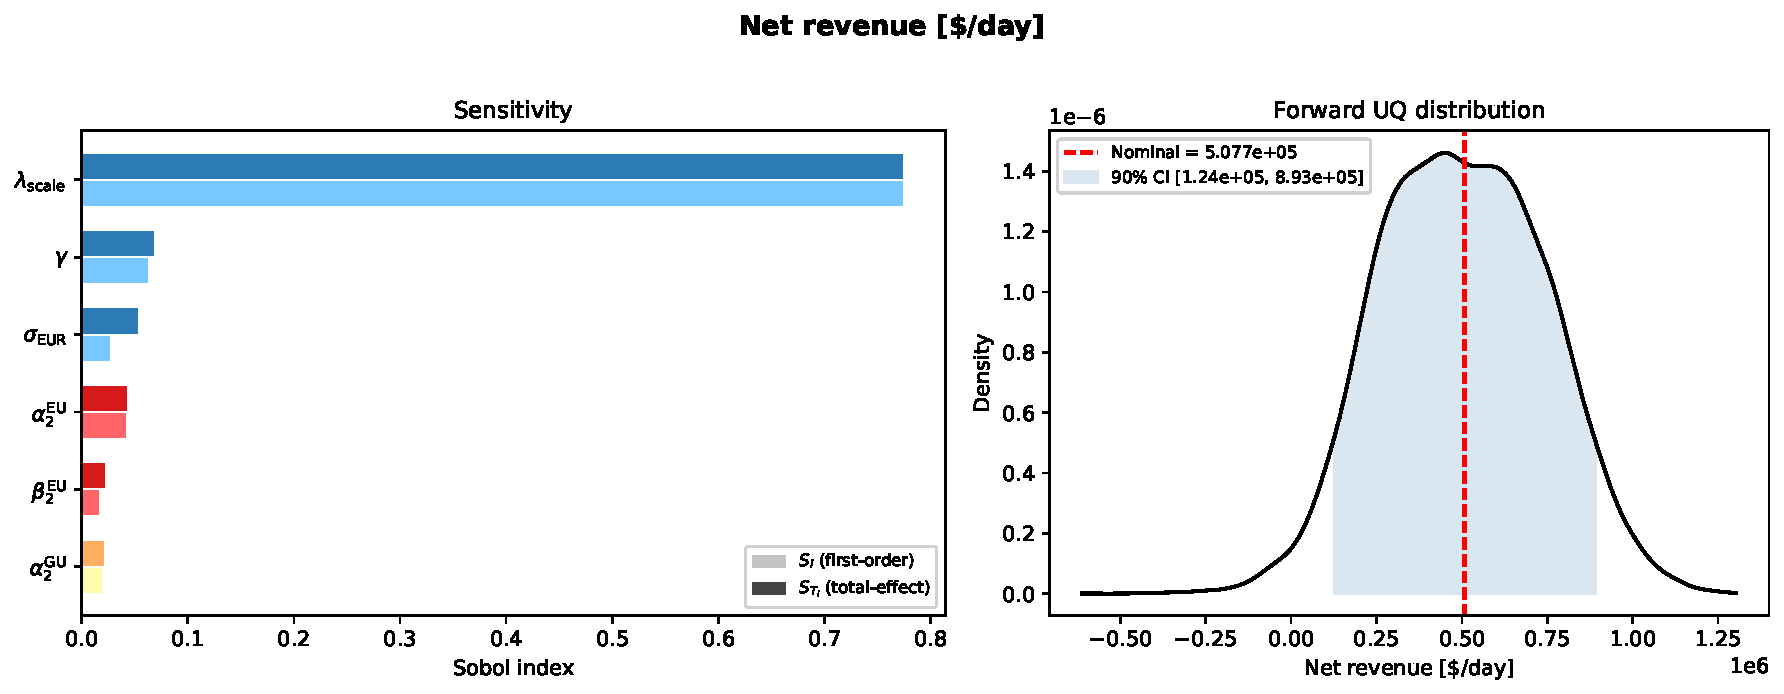
\includegraphics[width=\textwidth]{figures/fig_sa_qoi6.pdf}
  \caption{QoI~6: net revenue. Left: Sobol indices, dominated by $\lambda_{\text{scale}}$ ($S_{T_i} = 0.78$). Right: output distribution, with 90\% CI entirely positive.}
  \label{fig:sa-qoi6}
\end{figure}

The arrival rate scale $\lambda_{\text{scale}}$ dominates ($S_i = 0.78$, $S_{T_i} = 0.78$). Revenue is roughly proportional to total client flow, and $\lambda_{\text{scale}}$ scales all arrival rates across all three pairs. The model is nearly additive ($\sum S_i = 0.99$, $\sum S_{T_i} = 1.05$). Secondary contributors are $\gamma$ ($S_i = 0.06$, $S_{T_i} = 0.07$), $\alpha_2^{\text{EU}}$ ($S_i = 0.04$, $S_{T_i} = 0.04$), and $\sigma_{\text{EUR}}$ ($S_i = 0.03$, $S_{T_i} = 0.05$), along with $\alpha_2^{\text{GU}}$ and $\beta_2^{\text{EU}}$ at $S_{T_i} \approx 0.02$. This is the only QoI where GBP/USD demand parameters appear with nonzero Sobol indices, because net revenue sums contributions from all three pairs.

The forward UQ gives
\[
  \text{mean} = \$502\text{k/day}, \qquad \text{CV} = 48\%, \qquad 90\%\ \text{CI} = [\$124\text{k},\; \$893\text{k}]/\text{day}.
\]
The CI is entirely positive: the strategy is profitable across every parameter combination in the sample. The main source of revenue uncertainty is simply how much client flow the desk receives, not the risk management parameters.


% ==================================================================
\section{Discussion}
\label{sec:sa-discussion}

% ------------------------------------------------------------------
\subsection{Sensitivity structure}
\label{sec:sa-sensitivity-structure}

The central finding of the analysis is that different aspects of the market making strategy are sensitive to entirely different parameters. Table~\ref{tab:sa-summary} summarizes the dominant parameters and the degree of interaction for each QoI.

\begin{table}[ht]
\centering
\caption{Summary of the sensitivity structure. For each QoI, the dominant parameters (those with $S_{T_i} > 0.05$) and the presence of interactions ($\sum S_{T_i}$ relative to~1) are listed.}
\label{tab:sa-summary}
\begin{tabular}{@{}llc@{}}
\toprule
Quantity of interest & Dominant parameters & Interactions \\
\midrule
Tier spread differential (QoI~1) & $\beta_2^{\text{EU}}$, $\beta_1^{\text{EU}}$, $\alpha_2^{\text{EU}}$ & None \\
Own-inventory skew (QoI~2) & $\sigma_{\text{EUR}}$, $\gamma$, $\lambda_{\text{scale}}$ & Small \\
Cross-inventory skew (QoI~3) & $\rho$, $\gamma$, $\lambda_{\text{scale}}$, $\sigma_{\text{GBP}}$ & Small \\
Own-pair hedge rate (QoI~4) & $\sigma_{\text{EUR}}$, $\gamma$, $\lambda_{\text{scale}}$, $\eta^{\text{EU}}$ & Significant \\
Cross-hedge momentum (QoI~5) & $\sigma_{\text{EUR}}$, $\rho$, $\gamma$, $\lambda_{\text{scale}}$, $\sigma_{\text{GBP}}$ & Small \\
Net revenue (QoI~6) & $\lambda_{\text{scale}}$, $\gamma$, $\sigma_{\text{EUR}}$ & Small \\
\bottomrule
\end{tabular}
\end{table}

The separation falls along clear lines. The tier spread differential is a \emph{microstructure} quantity: it depends only on the shape of the client demand curves and is insensitive to market-level conditions. The inventory skew and hedge rate are \emph{risk management} quantities: they depend on volatility, risk preference, and market activity, with the hedge rate additionally sensitive to execution cost. The cross-pair quantities (QoIs~3 and~5) introduce the correlation~$\rho$ as a new dimension that does not appear for any own-pair quantity. Net revenue is dominated by a single parameter, the overall level of client flow.


% ------------------------------------------------------------------
\subsection{Robustness of the optimal strategy}
\label{sec:sa-robustness}

The forward uncertainty quantification reveals a gradient of robustness across the strategy's components. Table~\ref{tab:sa-forward-uq} summarizes the output distributions.

\begin{table}[ht]
\centering
\caption{Forward uncertainty quantification results. The coefficient of variation (CV) measures the relative spread of each output distribution. Sample size $2N = 20{,}000$.}
\label{tab:sa-forward-uq}
\begin{tabular}{@{}lcccc@{}}
\toprule
QoI & Mean & Std & 90\% CI & CV \\
\midrule
Tier spread diff.\ [bps]       & $-0.22$ & 0.09 & $[-0.37,\; -0.09]$ & 39\% \\
Own-inv.\ skew [bps]           & $0.15$ & 0.06 & $[0.07,\; 0.25]$ & 38\% \\
Cross-inv.\ skew [bps]         & $0.055$ & 0.026 & $[0.024,\; 0.105]$ & 46\% \\
Own-pair hedge [M\$/s]         & $-0.0335$ & 0.0372 & $[-0.107,\; 0]$ & 111\% \\
Cross-hedge mom.\ [decimal]    & $-1.17 \times 10^{-5}$ & $5.4 \times 10^{-6}$ & $[-2.2,\; -0.4] \times 10^{-5}$ & 46\% \\
Net revenue [\$/day]           & $502{,}000$ & 240{,}000 & $[124\text{k},\; 893\text{k}]$ & 48\% \\
\bottomrule
\end{tabular}
\end{table}

The quoting policy is relatively robust, with CVs of 38--46\% for the spread differential, own-inventory skew, and cross-inventory skew. These outputs are stable under parameter uncertainty: the spreads and inventory adjustments change, but not by an order of magnitude. The hedge rate is a different story. With a CV of 111\% and a 90\% CI spanning from $-0.108$ to 0\,M\$/s, the model's hedging prescription is highly uncertain. The distribution is heavily left-skewed because small values of~$\eta$ produce extremely large hedge rates through the $1/(2\eta)$ factor.

Figure~\ref{fig:sa-scatter-eta} makes this nonlinearity visible. The scatter plot of $\eta^{\text{EU}}$ versus the own-pair hedge rate shows the hyperbolic $1/\eta$ relationship: as $\eta$ decreases from $2 \times 10^{-5}$ to $0.5 \times 10^{-5}$, the hedge rate magnitude explodes from around $-0.012$ to beyond $-0.12$\,M\$/s. Underestimating market impact by a factor of two can lead to a factor-of-two overestimate of the optimal hedging rate.

\begin{figure}[ht]
  \centering
  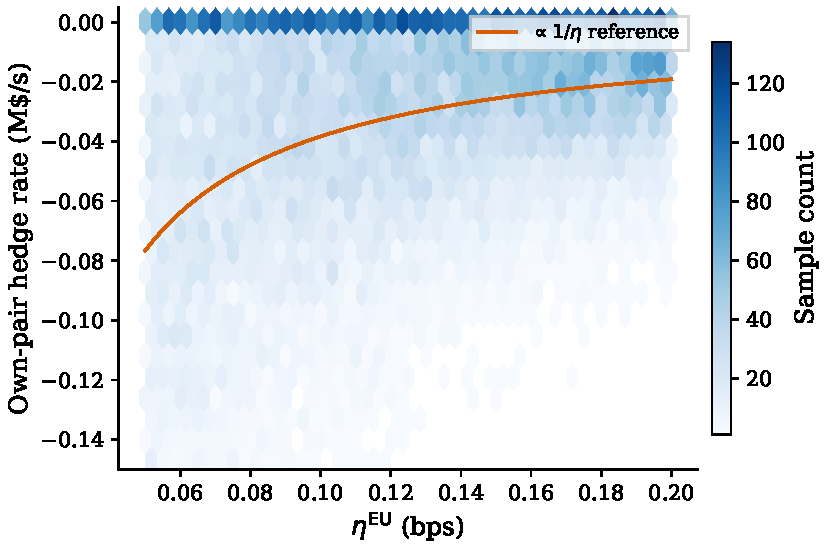
\includegraphics[width=0.6\textwidth]{figures/fig_sa_scatter_eta_hedge.pdf}
  \caption{Scatter plot of $\eta^{\text{EU}}$ versus the own-pair hedge rate ($n = 20{,}000$ samples). The red curve shows the $1/\eta$ reference scaling. The enormous spread at low~$\eta$ values reflects the multiplicative interaction with other parameters.}
  \label{fig:sa-scatter-eta}
\end{figure}

Figure~\ref{fig:sa-scatter-rho} illustrates a different type of sensitivity: the approximately linear relationship between~$\rho$ and the cross-inventory skew. As the correlation increases from 0.3 to 0.9, the cross-skew roughly doubles. This is consistent with the mechanism identified in Section~\ref{sec:sa-qoi3}: correlation controls the off-diagonal covariance $\Sigma_{\text{EUR,GBP}} = \rho\,\sigma_{\text{EUR}}\,\sigma_{\text{GBP}}$, which is the primary source of the cross-pair coupling in the Riccati equation. The vertical spread at each $\rho$ value reflects the combined effect of the other global parameters ($\gamma$, $\lambda_{\text{scale}}$, $\sigma_{\text{GBP}}$).

\begin{figure}[ht]
  \centering
  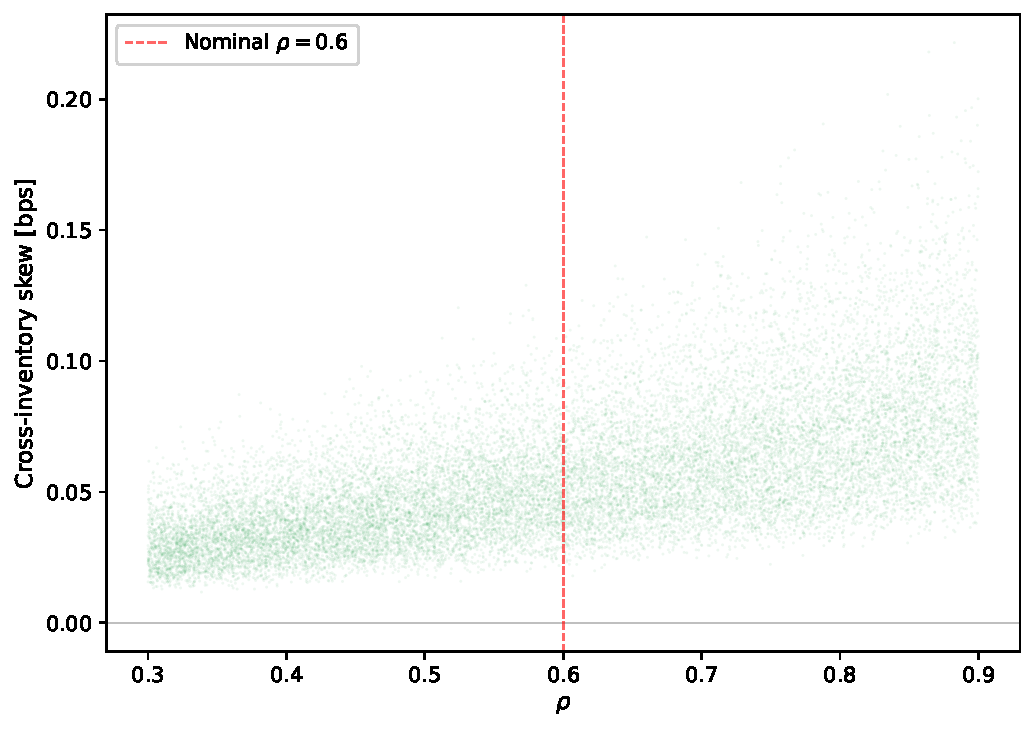
\includegraphics[width=0.6\textwidth]{figures/fig_sa_scatter_rho_cross.pdf}
  \caption{Correlation~$\rho$ versus cross-inventory skew ($n = 20{,}000$ samples). The linear fit confirms the approximately linear relationship: the cross-skew roughly doubles from low to high correlation.}
  \label{fig:sa-scatter-rho}
\end{figure}

The net revenue remains positive across the entire parameter space explored (90\% CI $= [\$124\text{k},\; \$893\text{k}]$/day). The strategy is profitable regardless of the parameter combination. The main risk under parameter uncertainty is not that the strategy loses money, but that the hedging prescriptions may be unreliable: the desk does not know how aggressively to hedge, even though it knows it will be profitable.


% ------------------------------------------------------------------
\subsection{Practical implications}
\label{sec:sa-practical}

The sensitivity analysis has concrete consequences for a desk deploying this model. The quoting policy is the most reliable component: with CVs of 38--46\%, the tier spreads and inventory skew the model produces are stable under parameter uncertainty. A desk can set its client-facing quotes from the model with reasonable confidence, even if the underlying parameters carry estimation error.

The hedging prescription is less reliable. With a CV of 111\%, the model's hedge rate is highly sensitive to the market impact parameter~$\eta$: the $1/(2\eta)$ factor means that small errors in the~$\eta$ estimate produce large swings in the prescribed hedging speed. The model identifies \emph{whether} to hedge and in \emph{which direction}, but the aggressiveness of hedging should be treated as a guide rather than a hard prescription. Real-time monitoring or trader oversight on hedging speed is warranted.

Calibration effort should be targeted accordingly. Each pair's quoting depends on its own demand curve parameters ($\alpha_n$, $\beta_n$), while the risk management quantities depend on the global parameters ($\sigma$, $\rho$, $\gamma$, $\lambda_{\text{scale}}$) and the own-pair execution cost~$\eta$. Cross-pair demand parameters have negligible effect. These two groups also evolve differently: the global parameters reflect market conditions that shift daily and benefit from frequent recalibration, while the demand curves describe client behavior and change more slowly. In particular, a desk should monitor the correlation~$\rho$ closely, as the cross-inventory effect on quoting roughly doubles between low and high correlation regimes (Figure~\ref{fig:sa-scatter-rho}), making cross-pair positions more relevant for quoting during correlated markets.

Despite the hedge rate uncertainty, the strategy's profitability is not in question. The net revenue 90\% CI is entirely positive (Table~\ref{tab:sa-forward-uq}). The risk under parameter uncertainty is not that the desk loses money, but that it hedges too aggressively or too passively, affecting the efficiency of the strategy rather than its sign.


% ------------------------------------------------------------------
\subsection{Connection to the PDE solution}
\label{sec:sa-bridge}

All results in this chapter are based on the ODE approximation, which replaces the exact Hamiltonians with quadratic Taylor expansions around zero quoting momentum. In Chapter~\ref{ch:pde}, we develop a grid-based PDE solver for the full HJB equation in the two-currency case and compare the ODE and PDE solutions across a range of parameter regimes. This comparison verifies whether the sensitivity conclusions derived here carry over to the exact solution, or whether the quadratic approximation introduces biases that alter the sensitivity structure.

\chapter{Grid-Based PDE Solver}
\label{ch:pde}

The ODE approximation developed in Chapter~\ref{ch:ode} is computationally attractive: the Riccati system scales quadratically in the number of currencies and can be solved in milliseconds. However, this efficiency comes at a cost. The quadratic ansatz $\hat\theta(t,y) = -y^\T A(t)\,y - y^\T B(t) - C(t)$ restricts the value function to a particular parametric family, and the Hamiltonian is replaced by its second-order Taylor expansion around $p = 0$. At large inventories, where the true value function deviates from a quadratic and the momentum $p$ entering the Hamiltonian is far from zero, the approximation may break down. To assess when and how this happens, we turn to a direct numerical solution of the HJB equation.

In the two-currency case ($d = 2$), the inventory state is two-dimensional and the PDE is amenable to grid-based methods. We develop a fully implicit Euler solver with policy iteration (Howard's algorithm) for the HJB equation derived in Chapter~\ref{ch:model}. The key numerical challenge is the extreme stiffness introduced by the hedging Hamiltonian, which amplifies value function gradients by a factor of order $10^8$. We address this through a monotone finite difference scheme that guarantees the discrete comparison principle required for convergence. With this scheme in place, the solver handles the original model parameters without any artificial regularisation.

This chapter is organised as follows. Section~\ref{sec:pde-domain} describes the computational domain and grid. Section~\ref{sec:pde-spatial} presents the spatial discretisation of each term in the HJB equation. Section~\ref{sec:pde-stiffness} analyses the stiffness structure and explains why explicit time stepping is infeasible. Section~\ref{sec:pde-implicit} develops the fully implicit solver, including the policy iteration algorithm and the monotone differencing scheme. Section~\ref{sec:pde-convergence} discusses convergence behaviour and computational cost. Finally, Section~\ref{sec:pde-results} compares the PDE and ODE solutions at nominal parameters and across the parameter regimes identified in Chapter~\ref{ch:sensitivity}.


% ==================================================================
\section{Computational domain}
\label{sec:pde-domain}

We work with the two-currency model (USD, EUR) from Table~1 of \cite{barzykin2023}. Since USD is the reference currency with $\sigma_{\text{USD}} = 0$, the effective state variables are the two inventory components $y = (y_{\text{USD}}, y_{\text{EUR}})$, measured in millions of USD. The PDE is solved on a uniform Cartesian grid
\begin{equation}
  \label{eq:grid}
  \Omega = [-Y_{\max}, Y_{\max}]^2, \qquad
  y_i^{(k)} = -Y_{\max} + k\,\Delta y, \quad k = 0, 1, \ldots, n-1,
\end{equation}
with $Y_{\max} = 150$~M\$, $\Delta y = 1$~M\$, and $n = 301$ grid points per axis. This gives a total of $N = 301^2 = 90{,}601$ grid points.

Two considerations determine these choices. First, the grid spacing $\Delta y = 1$~M\$ is chosen so that every trade size in the model ($z \in \{1, 5, 10, 20, 50\}$~M\$) is an exact multiple of $\Delta y$. This ensures that the shifted point $y + z\,d_{ij}$ appearing in the quoting Hamiltonian always falls on a grid node, avoiding the need for interpolation. Second, the domain extends 50~M\$ beyond the region of interest $[-100, 100]$~M\$ in each direction. This buffer accommodates the largest trade size ($z = 50$~M\$): without it, the quoting Hamiltonian at $|y| > 50$~M\$ would lose the $z = 50$ contribution, artificially degrading the solution in the interior.

The terminal condition is $\theta(T, y) = -y^\T \kappa\, y$, which equals zero everywhere since the paper sets $\kappa = 0$. At the domain boundary $\partial\Omega$, we do not impose Dirichlet conditions. Instead, quoting contributions whose shifted lookup $y + z\,d_{ij}$ falls outside $\Omega$ are simply dropped, acting as an implicit inventory limit. For the implicit solver (Section~\ref{sec:pde-implicit}), boundary rows in the linear system are set to identity, effectively freezing boundary values. This simple treatment suffices because the 50~M\$ buffer ensures that the solution in the region of interest is insensitive to boundary effects.


% ==================================================================
\section{Spatial discretisation}
\label{sec:pde-spatial}

We write the HJB equation in backward time $\tau = T - t$, so that it takes the form
\begin{equation}
  \label{eq:hjb-backward}
  \partial_\tau \theta = \underbrace{\frac{1}{2}\operatorname{Tr}\!\bigl(\mathcal{D}(y)\,\Sigma\,\mathcal{D}(y)\,D^2_{yy}\theta\bigr)}_{\text{diffusion}}
  - \underbrace{\frac{\gamma}{2}\,y^\T \Sigma\, y}_{\text{running penalty}}
  + \underbrace{Q(y, \theta)}_{\text{quoting}}
  + \underbrace{\mathcal{H}_{\text{hedge}}(y, \nabla_y\theta)}_{\text{hedging}},
\end{equation}
where we have used that the drift $\mu = 0$ in the paper's example. The right-hand side defines the spatial operator $F[\theta]$, which we now discretise term by term.


% ------------------------------------------------------------------
\subsection{Diffusion}
\label{sec:pde-diffusion}

The diffusion term involves the Hessian of $\theta$ weighted by the state-dependent volatility. Expanding the trace,
\begin{equation}
  \label{eq:diffusion-expanded}
  \frac{1}{2}\operatorname{Tr}\!\bigl(\mathcal{D}(y)\,\Sigma\,\mathcal{D}(y)\,D^2_{yy}\theta\bigr)
  = \frac{1}{2}\sum_{i=1}^d \Sigma_{ii}\,y_i^2\,\frac{\partial^2\theta}{\partial y_i^2}
  + \sum_{i < j} \Sigma_{ij}\,y_i\,y_j\,\frac{\partial^2\theta}{\partial y_i\,\partial y_j}.
\end{equation}
Since the reference currency has $\sigma_{\text{USD}} = 0$, the entire first row and column of $\Sigma$ vanish. In the two-currency case, only a single diagonal term survives:
\begin{equation}
  \label{eq:diffusion-2ccy}
  \frac{1}{2}\,\sigma_{\text{EUR}}^2\,y_{\text{EUR}}^2\,\frac{\partial^2\theta}{\partial y_{\text{EUR}}^2}.
\end{equation}
The second derivative is approximated by the standard central difference stencil
\begin{equation}
  \label{eq:central-2nd}
  \frac{\partial^2\theta}{\partial y_i^2}\bigg|_k \approx \frac{\theta_{k+1} - 2\,\theta_k + \theta_{k-1}}{\Delta y^2},
\end{equation}
using one-sided (forward or backward) stencils at the domain boundary. The boundary stencils are first-order accurate rather than second-order, but they lie in the buffer zone where solution quality is not critical.


% ------------------------------------------------------------------
\subsection{Running penalty}
\label{sec:pde-penalty}

The running penalty $-(\gamma/2)\,y^\T \Sigma\, y$ does not involve $\theta$ and is precomputed once on the grid. In the two-currency case, the only nonzero contribution is
\begin{equation}
  -\frac{\gamma}{2}\,\sigma_{\text{EUR}}^2\,y_{\text{EUR}}^2.
\end{equation}
This term enters the right-hand side of~\eqref{eq:hjb-backward} as a source that penalises large inventory positions, driving the value function downward at the grid boundary.


% ------------------------------------------------------------------
\subsection{Quoting Hamiltonian}
\label{sec:pde-quoting}

The quoting term evaluates the exact Hamiltonian rather than the quadratic Taylor approximation used in the ODE. For each directed currency pair $(i,j)$, client tier $n$, and trade size $z_k$, the contribution at inventory $y$ is
\begin{equation}
  \label{eq:quoting-contribution}
  z_k\,\lambda_k\,H^n\!\left(\frac{\theta(y) - \theta(y + z_k\,d_{ij})}{z_k}\right),
\end{equation}
where $d_{ij} = e_i - e_j$ is the direction vector of the trade (the market maker receives currency~$i$ and delivers currency~$j$), $\lambda_k$ is the arrival rate for size $z_k$, and
\begin{equation}
  \label{eq:H-exact}
  H^n(p) = \sup_\delta\; f^n(\delta)\,(\delta - p), \qquad f^n(\delta) = \frac{1}{1 + e^{\alpha_n + \beta_n\,\delta}},
\end{equation}
is the quoting Hamiltonian for the logistic intensity function $f^n$. As shown in Chapter~\ref{ch:ode}, the supremum admits a semi-closed form via the Lambert~$W$ function:
\begin{equation}
  \label{eq:H-lambert}
  H^n(p) = \frac{w}{\beta_n}, \qquad w = W_0\!\bigl(e^{-(1 + \alpha_n + \beta_n p)}\bigr),
\end{equation}
where $W_0$ denotes the principal branch. The full quoting term $Q(y, \theta)$ is the sum of~\eqref{eq:quoting-contribution} over all directed pairs, tiers, and sizes. In the paper's model, the trade sizes are discrete ($z_k \in \{1, 5, 10, 20, 50\}$~M\$), so no numerical quadrature is required.

The argument of $H^n$ in~\eqref{eq:quoting-contribution} involves the finite difference $(\theta(y) - \theta(y + z_k\,d_{ij}))/z_k$, which couples each grid point to a shifted neighbor at distance $z_k$ along the direction $d_{ij}$. Since $\Delta y$ divides all trade sizes, these shifted points lie exactly on the grid. When the shifted point falls outside $\Omega$, the corresponding contribution is set to zero — the market maker does not quote that size at that inventory. For the two-currency case with two directed pairs, two tiers, and five trade sizes, this gives $2 \times 2 \times 5 = 20$ quoting contributions per grid point, each coupling a grid point to one shifted neighbor.


% ------------------------------------------------------------------
\subsection{Hedging Hamiltonian}
\label{sec:pde-hedging}

For each canonical currency pair $(i,j)$ with $i < j$, the hedging Hamiltonian evaluates
\begin{equation}
  \label{eq:H-hedge}
  \mathcal{H}^{i,j}(p) = \sup_\xi\;\bigl(p\,\xi - \psi^{i,j}\,|\xi| - \eta^{i,j}\,\xi^2\bigr)
  = \frac{\bigl(\max(|p| - \psi^{i,j},\; 0)\bigr)^2}{4\,\eta^{i,j}},
\end{equation}
where $\psi^{i,j}$ and $\eta^{i,j}$ are the proportional spread cost and quadratic market impact for the D2D pair, and the argument is
\begin{equation}
  \label{eq:p-hedge}
  p^{i,j}(y) = \frac{\partial\theta}{\partial y_i} - \frac{\partial\theta}{\partial y_j}
  + k_i\,y_i\!\left(1 + \frac{\partial\theta}{\partial y_i}\right) - k_j\,y_j\!\left(1 + \frac{\partial\theta}{\partial y_j}\right).
\end{equation}
In the paper's example, the market impact parameters $k_i$ are negligibly small, so $p$ reduces to the difference of value function gradients along the two currency axes. The gradients are approximated by central finite differences in the grid interior.

The optimal hedge rate at the supremum is
\begin{equation}
  \label{eq:xi-star}
  \xi^*(p) = \begin{cases}
    (p - \psi) / (2\eta) & \text{if } p > \psi, \\
    (p + \psi) / (2\eta) & \text{if } p < -\psi, \\
    0 & \text{if } |p| \leq \psi.
  \end{cases}
\end{equation}
The dead zone $|p| \leq \psi$ reflects the fact that the proportional spread cost makes small hedges unprofitable. Outside the dead zone, the optimal hedge rate is proportional to $1/(2\eta)$, which is of order $5 \times 10^8$ for the paper's parameters. This extreme sensitivity to the value function gradient is the dominant source of numerical stiffness, as we discuss in the next section.

Once the optimal hedge rate $\xi^*$ is computed, the hedging contribution to the right-hand side of~\eqref{eq:hjb-backward} can be decomposed into a term involving $\xi^*\,\nabla_y\theta$ (an advection-like coupling to the value function) and a source term collecting the execution costs $-\psi\,|\xi^*| - \eta\,(\xi^*)^2$. This decomposition is central to the linearised system in the implicit solver.


% ==================================================================
\section{Stiffness and the need for implicit time stepping}
\label{sec:pde-stiffness}

The simplest approach to marching~\eqref{eq:hjb-backward} forward in $\tau$ is explicit Euler:
\begin{equation}
  \label{eq:explicit-euler}
  \theta^{m+1} = \theta^m + \Delta t\; F[\theta^m],
\end{equation}
where $F$ is the spatial operator. Explicit time stepping has the virtue of simplicity — each step requires only one evaluation of $F$ — but it is subject to stability constraints.

The diffusion term imposes the standard CFL condition $\Delta t < \Delta y^2 / (\sigma^2\,Y_{\max}^2)$. With the paper's parameters ($\sigma_{\text{EUR}} = 80$~bps, $Y_{\max} = 150$~M\$, $\Delta y = 1$~M\$), this yields $\Delta t < 0.69$~days, which is very generous relative to the time horizon $T = 0.05$~days. The diffusion is not the binding stability constraint.

The hedging Hamiltonian, however, introduces severe stiffness. The gain $1/(4\eta) \approx 2.5 \times 10^8$ in~\eqref{eq:H-hedge} means that even modest value function gradients produce enormous Hamiltonian values, creating a positive feedback loop: a small perturbation in $\theta$ amplifies the gradient, which amplifies $\mathcal{H}_{\text{hedge}}$, which amplifies $\theta$ further. This mechanism causes numerical blow-up regardless of how small $\Delta t$ is chosen, because the nonlinear Hamiltonian does not satisfy a standard linear CFL condition.

An intermediate approach --- treating the diffusion term implicitly while keeping the Hamiltonians explicit (an IMEX or semi-implicit scheme) --- was also considered. Since the stability constraint is dominated by the hedging Hamiltonian rather than the diffusion, this scheme requires the same artificial scaling of $\eta$ as the explicit method and offers no improvement. The stiffness can only be resolved by treating the hedging term implicitly, which leads naturally to a fully implicit scheme.


% ==================================================================
\section{Fully implicit solver with policy iteration}
\label{sec:pde-implicit}


% ------------------------------------------------------------------
\subsection{Implicit Euler formulation}
\label{sec:pde-implicit-euler}

The fully implicit Euler scheme reads
\begin{equation}
  \label{eq:implicit-euler}
  \theta^{m+1} - \Delta t\; F[\theta^{m+1}] = \theta^m.
\end{equation}
This is a nonlinear equation for $\theta^{m+1}$, because the spatial operator $F$ contains the quoting and hedging Hamiltonians, which involve suprema over controls. In return for this added complexity, the implicit scheme avoids the CFL restriction: the stiff hedging term is absorbed into the left-hand side and handled by the linear algebra solver.


% ------------------------------------------------------------------
\subsection{Policy iteration}
\label{sec:pde-pi}

We solve the nonlinear equation~\eqref{eq:implicit-euler} at each time step using policy iteration (Howard's algorithm), which alternates between two steps:

\begin{enumerate}
  \item \textbf{Fix the controls.} Given a current estimate $\theta^k$ (initialised to $\theta^m$), compute the optimal quotes $\delta^*(y)$ and hedge rates $\xi^*(y)$ at every grid point using the formulas~\eqref{eq:H-lambert} and~\eqref{eq:xi-star}.

  \item \textbf{Solve the linearised system.} With the controls frozen, the suprema in $F$ are removed and the operator becomes linear in $\theta^{k+1}$. This yields a sparse linear system
  \begin{equation}
    \label{eq:linearised-system}
    (I - \Delta t\,A)\;\theta^{k+1} = \theta^m + \Delta t\; s,
  \end{equation}
  where $A$ is a sparse matrix encoding how each grid point's value depends on its neighbours through finite differences, and $s$ is a source vector collecting all terms that do not depend on $\theta^{k+1}$.
\end{enumerate}

The iteration terminates when the relative change falls below a prescribed tolerance:
\begin{equation}
  \frac{\|\theta^{k+1} - \theta^k\|_\infty}{\max(1,\;\|\theta^{k+1}\|_\infty)} < \varepsilon_{\text{PI}}.
\end{equation}
Policy iteration is equivalent to Newton's method applied to the Bellman equation and inherits its quadratic convergence rate, typically requiring only a small number of iterations per time step.


% ------------------------------------------------------------------
\subsection{Assembly of the linearised system}
\label{sec:pde-assembly}

With the controls frozen, each term in the spatial operator~\eqref{eq:hjb-backward} contributes either to the sparse matrix $A$ (through its dependence on $\theta^{k+1}$) or to the source vector $s$ (through quantities known from the current iterate $\theta^k$). We now describe these contributions.

The \emph{running penalty} $-(\gamma/2)\,y^\T \Sigma\,y$ has no $\theta$ dependence and enters entirely as a source term. It is precomputed once on the grid.

The \emph{diffusion} term is linear in $\theta$ and enters entirely into $A$. For each axis $i$ with $\Sigma_{ii} > 0$, the central difference stencil~\eqref{eq:central-2nd} contributes three entries per row: $\theta_{k-1}$, $\theta_k$, and $\theta_{k+1}$ along axis $i$, weighted by $\frac{1}{2}\,\Sigma_{ii}\,y_i^2 / \Delta y^2$.

The \emph{quoting Hamiltonian} requires more care. With the optimal markup $\delta^*$ and fill probability $f^*$ frozen, the contribution of a single quoting event $(n, i, j, z_k)$ at grid point $y$ is
\begin{equation}
  z_k\,\lambda_k\,f^*\!\left(\delta^* - \frac{\theta(y) - \theta(y + z_k\,d_{ij})}{z_k}\right)
  = \underbrace{z_k\,\lambda_k\,f^*\,\delta^*}_{\to\; s}
  \;-\; \underbrace{\lambda_k\,f^*\,\bigl(\theta(y) - \theta(y + z_k\,d_{ij})\bigr)}_{\to\; A}.
\end{equation}
The first part is a source term (the expected profit per quoting event). The second part contributes two entries per row of $A$: a diagonal entry $-\lambda_k\,f^*$ and an off-diagonal entry $+\lambda_k\,f^*$ at the shifted position $y + z_k\,d_{ij}$. With 20 quoting contributions in the two-currency case, this adds up to 40 off-diagonal entries per row.

The \emph{hedging Hamiltonian} with frozen hedge rate $\xi^*$ decomposes into a source term $-\psi\,|\xi^*| - \eta\,(\xi^*)^2$ (the execution cost) and a linear term $\xi^*\,(\partial\theta/\partial y_i - \partial\theta/\partial y_j)$ (the advection coupling). The advection term contributes to $A$ through the gradient stencil, adding up to four entries per row (two per axis). The discretisation of this gradient is the subject of the next subsection.

In total, the matrix $I - \Delta t\,A$ has approximately 48 nonzero entries per row, giving roughly $4.3 \times 10^6$ nonzeros for the $90{,}601 \times 90{,}601$ system. The matrix is assembled in COO format and converted to CSR for the sparse direct solve.


% ------------------------------------------------------------------
\subsection{Monotone differencing and the M-matrix property}
\label{sec:pde-monotone}

The hedging advection term $\xi^*\,\partial\theta/\partial y_i$ is a first-order transport-like operator with velocity $v = \xi^*(y)$. For the paper's parameters, $|\xi^*|$ can reach $50{,}000$~M\$/day outside the dead zone, producing matrix entries of magnitude $\Delta t\,|\xi^*|/\Delta y \approx 60$ when central differences are used for the gradient. Since the diagonal entry from this term is zero under central differencing, and the identity contributes only~1 to the diagonal, the matrix $I - \Delta t\,A$ loses diagonal dominance. The resulting linear system is ill-conditioned, and the sparse direct solver produces erroneous solutions that cause policy iteration to diverge.

The remedy is to use directional (upwind) differences for the hedging gradient, chosen so that the matrix $I - \Delta t\,A$ is an \emph{M-matrix}: a matrix with non-positive off-diagonal entries and a dominant positive diagonal. Specifically, for the advection operator $+v\,\partial\theta/\partial y_i$ entering the right-hand side of~\eqref{eq:hjb-backward}, we discretise as
\begin{equation}
  \label{eq:upwind}
  v\,\frac{\partial\theta}{\partial y_i}\bigg|_k \approx \begin{cases}
    v\,(\theta_{k+1} - \theta_k) / \Delta y & \text{if } v > 0, \\
    v\,(\theta_k - \theta_{k-1}) / \Delta y & \text{if } v < 0.
  \end{cases}
\end{equation}
Under this choice, the contributions to $I - \Delta t\,A$ from the hedging gradient are:
\begin{alignat}{2}
  &\text{diagonal:}      &\quad &{+}\;\Delta t\,|v|/\Delta y, \label{eq:upwind-diag} \\
  &\text{off-diagonal:}  &\quad &{-}\;\Delta t\,\max(v, 0)/\Delta y \;\;\text{(at $k+1$)}, \notag \\
  &                      &\quad &{+}\;\Delta t\,\min(v, 0)/\Delta y \;\;\text{(at $k-1$)}. \notag
\end{alignat}
The diagonal entry is always positive, and both off-diagonal entries are non-positive, regardless of the sign or magnitude of $v$. Combined with the positive contributions from the identity and the diffusion operator, this guarantees that $I - \Delta t\,A$ is an M-matrix.

We note that the upwind direction in~\eqref{eq:upwind} is the opposite of the standard convention for the transport equation $\partial_\tau u + v\,\partial u/\partial y = 0$, where $v > 0$ calls for a backward difference. The difference arises because the advection term in~\eqref{eq:hjb-backward} enters with a positive sign on the right-hand side: positive $v\,\partial\theta/\partial y$ makes $\theta$ grow, and the implicit scheme must move this growth to the left-hand side with the correct sign to maintain the M-matrix structure.

The M-matrix property is significant for two reasons. First, it ensures a discrete comparison principle: if two solutions satisfy an ordering at the boundary and in the source, the ordering is preserved in the interior. This is the discrete analogue of the maximum principle for elliptic PDEs, and it is a necessary condition for the convergence of monotone numerical schemes in the framework of Barles and Souganidis~\cite{barles1991}. Second, it guarantees the convergence of policy iteration, which relies on the monotonicity of the discrete Bellman operator. Without the M-matrix structure, policy iteration may oscillate or diverge even when the continuous problem is well-posed.

The price of monotone differencing is a reduction in spatial accuracy from second order (central differences) to first order. In practice, this loss is confined to the hedging gradient and is most noticeable at the grid boundary, where the first-order stencil interacts with the boundary treatment. In the interior of the grid, where the solution is smooth and the region of interest lies, the first-order error is small relative to the time discretisation error. The central difference stencils for the diffusion operator and the quoting Hamiltonian are unaffected.


% ==================================================================
\section{Convergence and computational cost}
\label{sec:pde-convergence}

With the monotone differencing scheme in place, the solver handles the paper's original parameters ($\eta = 10^{-9}$ in decimal units) without any artificial scaling or continuation. A tolerance of $\varepsilon_{\text{PI}} = 10^{-4}$ is used for the policy iteration. Detailed iteration traces reveal the following convergence pattern:

At the first time step (cold start from $\theta(T) = 0$), the policy iteration requires approximately 7 inner iterations. The relative change drops rapidly from $3.6 \times 10^{-2}$ to $2.8 \times 10^{-4}$ over the first five iterations, with the value at the origin $\theta(0,0)$ stabilising after iteration~5. The residual then stalls at approximately $2.5 \times 10^{-5}$, oscillating without further decrease. This stall is caused by the first-order accuracy of the upwind stencil at boundary points and does not affect the solution in the region of interest. Setting $\varepsilon_{\text{PI}} = 10^{-4}$, safely above the stall level, allows the iteration to terminate promptly.

At subsequent time steps, the previous solution provides an effective warm start, and the policy iteration converges in 2--4 inner iterations. With 20 time steps over the horizon $T = 0.05$~days, the solver completes in approximately 9~minutes on a $301 \times 301$ grid, with each sparse linear solve taking roughly 0.1~seconds via a direct sparse factorisation.

We remark that a continuation method in $\eta$ (solving a sequence of problems with decreasing $\eta$, using each solution to warm-start the next) was also tested. The monotone scheme alone was found to be sufficient for convergence at the original $\eta$, and the continuation added computational cost without improving the solution. This is consistent with the analysis in Section~\ref{sec:pde-monotone}: the stability issue is not the magnitude of $\eta$ per se, but the loss of the M-matrix property under central differencing.


% ==================================================================
\section{Numerical results}
\label{sec:pde-results}

We now compare the PDE solution against the ODE approximation from Chapter~\ref{ch:ode}. The comparison focuses on the three quantities of interest introduced in Chapter~\ref{ch:sensitivity}: the neutral spread $\delta^*(y = 0)$, the inventory skew $\delta^*(y = 10) - \delta^*(y = 0)$, and the hedge rate $\xi^*(y = 10)$.


% ------------------------------------------------------------------
\subsection{Nominal parameters}
\label{sec:pde-nominal}

At the paper's nominal parameter values, the PDE and ODE value functions agree closely. Along inventory slices through the origin, the two solutions are visually indistinguishable over the range $|y| \leq 100$~M\$. The maximum absolute difference is approximately $1.1 \times 10^{-4}$ in the value function, occurring at $|y_{\text{EUR}}| \approx 75$~M\$, compared to a typical value of $\theta(0,0) \approx 1.06 \times 10^{-2}$. This corresponds to a relative discrepancy of roughly 1\%.

The PDE value function is systematically higher than the ODE approximation at large inventories. The ODE relies on two coupled simplifications: a quadratic Taylor expansion $\hat{H}(p) \approx \alpha_0 + \alpha_1\,p + \frac{1}{2}\,\alpha_2\,p^2$ of the Hamiltonian and a quadratic ansatz $\hat\theta = -y^\T A\,y - y^\T B - C$ for the value function. Their combined effect is to slightly underestimate the true value at large $|y|$ --- the PDE, which captures the full nonlinear structure of both $H$ and $\theta$, shows that the market maker extracts marginally more value from quoting at extreme inventories than the ODE predicts.

% TODO: Add figure — PDE vs ODE value function along EUR inventory slice
% \begin{figure}[ht]
%   \centering
%   \includegraphics[width=0.8\textwidth]{figures/pde_ode_value_function.pdf}
%   \caption{Value function $\theta(0, y)$ along the EUR inventory axis ($y_{\text{USD}} = 0$) at $t = 0$, computed by the PDE solver (solid) and the ODE approximation (dashed). The inset shows the difference $\theta_{\text{PDE}} - \theta_{\text{ODE}}$.}
%   \label{fig:pde-ode-value}
% \end{figure}

The three quantities of interest confirm this picture. At the origin, the neutral spread and inventory skew from the PDE match those from the ODE to within the resolution of the grid. The hedge rate, which depends on the value function gradient rather than its level, also agrees well. These results confirm that the ODE approximation is accurate for the paper's nominal parameter set, consistent with the brief validation reported in~\cite{barzykin2023}.


% ------------------------------------------------------------------
\subsection{Sensitivity across parameter regimes}
\label{sec:pde-sensitivity}

The sensitivity analysis in Chapter~\ref{ch:sensitivity} identified four parameters that drive the quantities of interest: $\sigma_{\text{EUR}}$, $\gamma$, $\lambda_{\text{scale}}$, and $\eta$. To assess whether the ODE approximation remains reliable across their uncertainty ranges, we solve the PDE at the low and high end of each parameter's range (Table~\ref{tab:sensitivity-ranges} in Chapter~\ref{ch:sensitivity}), with all other parameters held at their nominal values. This produces 9~PDE solves in total: one at the nominal point and two for each of the four parameters.

% TODO: Add table — PDE vs ODE QoIs at each parameter configuration
% \begin{table}[ht]
%   \centering
%   \caption{Quantities of interest from the PDE and ODE solvers at nominal parameters and at the edges of the sensitivity ranges for $\sigma$, $\gamma$, $\lambda$, and $\eta$.}
%   \label{tab:pde-ode-qois}
%   \begin{tabular}{l rrr rrr}
%     \toprule
%     & \multicolumn{3}{c}{ODE} & \multicolumn{3}{c}{PDE} \\
%     \cmidrule(lr){2-4} \cmidrule(lr){5-7}
%     Config & $\delta^*(0)$ & skew & $\xi^*$ & $\delta^*(0)$ & skew & $\xi^*$ \\
%     \midrule
%     nominal & & & & & & \\
%     $\sigma$ low & & & & & & \\
%     $\sigma$ high & & & & & & \\
%     \ldots & & & & & & \\
%     \bottomrule
%   \end{tabular}
% \end{table}

For each parameter configuration, we compare the PDE and ODE values of the three quantities of interest, as well as the sensitivity magnitudes (the change in each QoI between the low and high parameter values). This comparison tests two things: whether the ODE accurately captures the absolute level of each QoI across parameter regimes, and whether it correctly predicts the direction and magnitude of the sensitivity.

% TODO: Add figure — bar chart comparing ODE vs PDE sensitivities
% \begin{figure}[ht]
%   \centering
%   \includegraphics[width=\textwidth]{figures/pde_ode_sensitivity_comparison.pdf}
%   \caption{Sensitivity of the three quantities of interest to the four key parameters, as computed by the PDE solver and the ODE approximation. Each bar shows the difference in the QoI between the high and low parameter values.}
%   \label{fig:pde-ode-sensitivity}
% \end{figure}


% ------------------------------------------------------------------
\subsection{Discussion}
\label{sec:pde-discussion}

The comparison across parameter regimes serves two purposes within the thesis. First, it validates the PDE solver itself: if the PDE and ODE solutions agree in regimes where the quadratic approximation is expected to be accurate, this provides confidence that the spatial operators and the implicit scheme are implemented correctly. Second, it validates the ODE-based sensitivity conclusions from Chapter~\ref{ch:sensitivity}: if the PDE confirms the same sensitivity rankings and magnitudes, it justifies using the computationally cheap ODE for the full uncertainty quantification study, including potential extensions to more than two currencies where the PDE becomes infeasible.

Any systematic discrepancies between the PDE and ODE solutions are most likely to appear in two regimes. First, at high volatility or high risk aversion, the optimal inventory skew increases, pushing the value function further from the quadratic form and the momentum $p$ further from zero, where the Taylor expansion of $H$ is least accurate. Second, at low $\eta$, the hedging Hamiltonian's gain $1/(4\eta)$ is largest, amplifying any differences in the value function gradient. In both cases, the PDE provides the more reliable benchmark, and the magnitude of the discrepancy characterises the domain of validity of the ODE approximation.

%\input{chapters/conclusion}

% --- Back matter ---
\backmatter

\printbibliography[heading=bibintro, title={References}]

% \appendix
% \input{chapters/appendix}

\end{document}